\chapter{Rare earth element distributions and trends in natural waters with a focus on groundwater}
\chaptermark{REE in natural waters}

This chapter is adapted from a publication by the same name, co-authored by David A. Dzombak and Athanasios K. Karamalidis.
This paper is citable as: 

Noack, C. W.; Dzombak, D. A.; Karamalidis, A. K., Rare Earth Element Distributions and Trends in Natural Waters with a Focus on Groundwater. \textit{Environ. Sci. Technol.} \textbf{2014}, \textit{48}, (8), 4317-4326.

My contributions to this work were the collection, analysis, and visualization of the data; development of \texttt{R} scripts; interpretation of results; and drafting of the manuscript.

\clearpage

\section*{Abstract}
Systematically varying properties and reactivities have led to focused research of the environmental forensics capabilities of the rare earth elements (REE).
Increasing anthropogenic inputs to natural systems may permanently alter the natural signatures of REEs, motivating characterization of natural REE variability.
We compiled and analyzed reported dissolved REE concentration data over a wide range of natural water types (groundwater, ocean-, river-, and lake water) and groundwater chemistries (e.g. fresh, brine, and acidic) with the goal of quantifying the extent of natural REE variability, especially for groundwater systems.
Quantitative challenges presented by censored data were addressed with non-parametric distributions and regressions.
Reported measurements of rare earth elements in natural waters range over nearly ten orders of magnitude, though the majority of measurements are within two to four orders of magnitude, and are highly correlated with one another.
Few global correlations exist among dissolved abundance and bulk solution properties in groundwaters indicating the complex nature of source-sink terms and the need for care when comparing results between studies.
This collection, homogenization, and analysis of a disparate literature facilitates inter-study comparison and provides insight into the wide range of variables that influence REE geochemistry.


\section{Introduction}

In the natural sciences, predictable thermodynamic differences between the rare earth elements (REE) allow for interpretation of natural geologic and chemical processes \citep{REE_dep_study, REE_soil_tracers}. 
Rare earth lithogeochemistries have long been used to infer depositional environments of geologic strata \citep{REE_dep_study, PAAS, Hanson_EPS_1980}.
Similarly, REE serve as benign analogs to the transuranic actinides for nuclear waste disposal studies \citep{Krauskopf_CG_1986, Millero_GCA_1992} and for studying mixing and metal cycling in the oceans \citep{DeBaar_Nat_1983, Elderfield_PTRS_1988}.
These characteristics make REE attractive tools for environmental forensic applications such as pollutant source identification and apportionment \citep{Kulkarni_AE_2006, Kulkarni_EST_2007}.

Based on atomic number, the REE are segregated into light and heavy REE (LREE and HREE, respectively) with the division occurring between Eu and Gd \citep{Castor_Hedrick};
some studies also distinguish middle REE (MREE), though the specific elements are inconsistently defined between authors \citep{Hannigan_CG_2001, Tang_CG_2010, Choi_CG_2009, Brookins_RMG_1989}.
These ``weight'' distinctions allow for simplified description and quantification of the inter-element relationships, typically ratios of normalized concentrations, which are exploited in REE analysis.
Similarly, anomalies of certain REE -- due to redox lability for Ce and Eu \citep{Brookins_RMG_1989} and large anthropogenic emissions for Gd \citep{Bau_EPSL_1996} -- are used to interpret geochemical processes. 
Y and Sc exhibit similar properties to the lanthanides and are thus included in the suite of REE with Y being most similar to HREE and Sc being most similar to LREE in solution \citep{Brookins_RMG_1989}.
 
Aquatic geochemists apply the same principles used by geologists, the inter-element ratios and anomalies described previously, to infer water-rock interactions, hydrologic connectivity between geologic units, and groundwater mixing members \citep{Johannesson_GCA_1997, Johannesson_GW_1997, BwireOjiambo_AG_2003, Siebert_AG_2012}.
Interactions with different mineral phases have been shown to alter REE patterns predictably.
For example, an MREE enrichment is observed for fresh waters in contact with phosphate-rich minerals \citep{Hannigan_CG_2001} while HREE enrichment is found in carbonate-rich waters \citep{Johannesson_EPSL_1996}.
Tester et al. \citep{Tesmer_HJ_2007} showed that groundwater end-members, especially at shallow depths, could be established by interpretation of REE patterns.
Similarly, REE concentrations have been used to calculate end-member contributions to groundwater \citep{Johannesson_GCA_1997, BwireOjiambo_AG_2003}.
 
The capabilities of REE to serve as tracers of groundwater migration and mixing have potential applications to the study of hydrology and geochemistry of shale gas development or the capture and sequestration of carbon dioxide (CO$_2$) gas in geologic formations.
For example, characteristic REE profiles could possibly enable detection of brines displaced from shale or CO$_2$ storage zones and into overlying groundwater aquifers \citep{Benson_Cole, Karamalidis_EST_2012, Chaudhuri_JOCGS_2011, Cheung_IJCG_2009}.
Capable tools for contaminant detection, as well as contaminant source apportionment, are critical to the long-term environmental feasibility of these technologies.
Increasing anthropogenic inputs of REE to the environment threaten to obfuscate natural signals, which would complicate these applications \citep{Kulaksiz_EI_2011, Kulaksiz_EPSL_2013}.

A primary challenge in analyzing REE data, like other geochemical compositional data \citep{Palarea_CompData_2011}, is the prevalence of censored observations, defined as values below the analytical method detection limit (MDL) or a value excluded due to excessive analytical interferences.
Appropriate statistical methodologies, largely borrowed from survival analysis (or reliability analysis), allow for analysis of these data without relying on substitution or interpolation \citep{Helsel_EST_1995}.
Utilizing these techniques removes the bias of left-censored data and of uneven sample sizes from summary statistics and statistical inference \citep{Helsel_EST_1995, Helsel_EST_2005}. 

Significant contributions to the understanding of REE geochemistry in natural waters have been made through critical review of thermodynamics \citep{Brookins_RMG_1989, Wood_CG_1990},
catchment-scale case studies \citep{Dia_GCA_2000, Gruau_WR_2004, Pourret_AG_2010, Ma_CG_2011},
and groundwater flow system studies \citep{Johannesson_GCA_1997, Johannesson_GCA_1999, Johannesson_CG_2000, Tang_CG_2006, Willis_CG_2011} among others.
Lacking thus far in the REE literature is the aggregation and analysis of the numerous and disparate studies of the REE and the origin of their concentrations.
Such a compilation would enhance inter-study comparison through internal consistency, allow for investigation of broader trends, and enhance statistical analysis by increasing sample sizes.

In this work, a compilation and analysis of data from independent studies of REE in natural waters was performed, focusing on trends in groundwaters.
The study focused on shallow groundwaters well as some deeper groundwaters capable of impacting surface water or shallow groundwater.
The compiled data were used to develop a consistent database of REE concentrations and their associated major solute chemistry and to explore interelement relationships, examine trends in REE abundance, and test hypotheses related to REE abundance as functions of major solution chemistry parameters.
The objectives of this work were: (1) to ascertain an expected range of dissolved REE concentrations in waters of variable chemistries, deriving unbiased estimates of REE distributions and (2) to investigate trends in REE abundance in groundwater in relation to other available chemical parameters (e.g. pH, ionic strength, and major solution species).

\section{Methods}

\subsection{Data assimilation and criteria}

The low-temperature, aqueous REE systematics were investigated by extracting available REE concentration data in reported studies of ground-, sea-, river-, and lake waters.
Data were gathered from these studies for dissolved REE concentrations (defined here as constituents passing through a 0.45 \si{\um} filter). 
Many studies filter at finer pore sizes in order to study colloidal association \citep{Dia_GCA_2000, Pourret_JCIS_2007, Stolpe_GCA_2013},
however 0.45 \si{\um} was chosen because it is a common size for groundwater analysis and  maximized the number of samples available.
While REE are commonly defined to include Y and Sc, very few studies measured Y and almost none examined Sc.
Therefore, our analyses of REE focused on the 14 naturally abundant lanthanides (excluding the short-lived, radioactive Pm).
In total, 31 studies with 619 samples were collected for groundwater,14, 19, 20, 22, 33-35, 37-40, 43-63
16 studies with 178 samples for seawater,7, 45, 64-77
16 studies with 259 samples for river water,12, 19, 48, 67, 71, 78-89
and 8 studies with 74 samples for lake water.19, 56, 57, 82, 85, 90-92

A significant literature exists for other water types, for example mine drainage \citep{Borrego_HR_2012, Bozau_AG_2004, Doulati_JEE_2013, Romero_AG_2010, Verplank_AG_2004, Worrall_GCA_2001, Zhao_IJCG_2007} and hydrothermal waters/hot springs \citep{Haas_GCA_1995, Lepel_conf_1988, Michard_GCA_1989, Lewis_GCA_1997, Lewis_GCA_1998, Sanada_Geotherm_2006}.
However, these water types have been excluded from this study in order to focus on waters minimally impacted by anthropogenic activity (in the case of mine drainage) and that occur broadly with chemistry dominated by near-surface pressure, temperature, and mineralogical conditions (in the case of hydrothermal waters/hot springs).

\subsection{Analysis of censored data}

In the accumulated dataset, 18\% of all REE measurements were either below detection or missing.
For individual elements in different waters, up to 52\% of measurements were censored (Tm in groundwater).
The censoring rates of each element, in each water type, are given in Figure~\ref{fig:cen_frac}.
Given this high frequency, it was necessary to employ modified statistical methods to handle this type of information31 and avoid creating a false data signal either by substitution (i.e., one-half MDL) or interpolation.

\begin{figure}[htbp]
\begin{center}
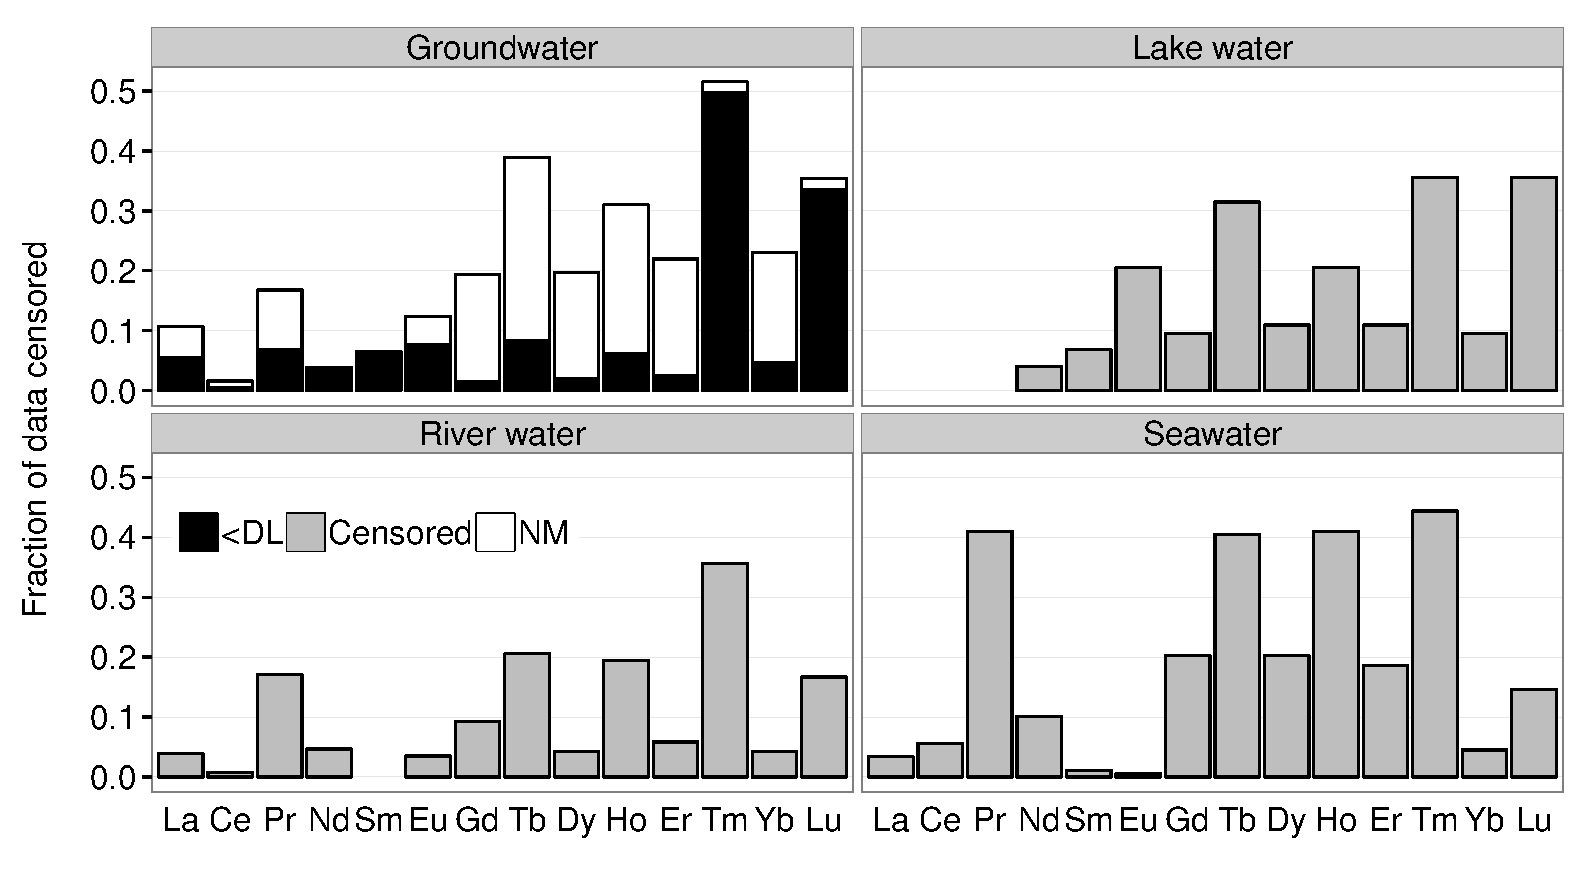
\includegraphics[width=\textwidth]{Ch3_figures/REE-waters-nonDet-type.pdf}
\caption{Fraction of below detection limit ($<$DL) or missing data (NM) for 14 REE in data sets for water types studied. For water types other than groundwater, censored data were not differentiated as below detection or missing, and are lumped together as ``censored''.}\label{fig:cen_frac}
\end{center}
\end{figure}


An additional complexity of this data set was the uneven distribution of data points between data sets (Figure~\ref{fig:sample_dist}).
For example, some data sets included more than seventy samples, while other contained fewer than ten.
This uneven distribution can bias calculated statistics towards studies with a higher number of samples, giving larger studies more weight than smaller studies \citep{Singh_JAWMA_2013}.

\begin{figure}[htbp]
\begin{center}
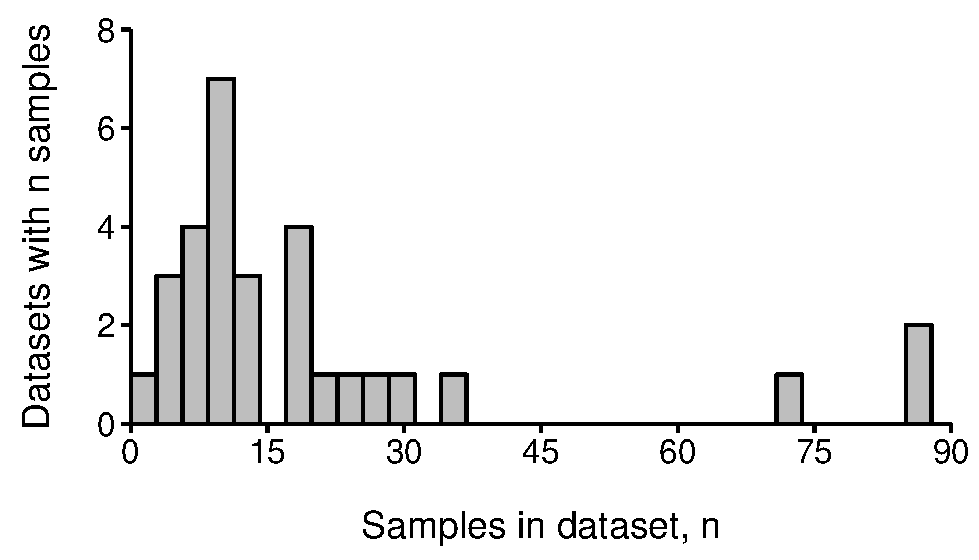
\includegraphics[width=0.8\textwidth]{Ch3_figures/cite-n-dist.pdf}
\caption{Histogram of sample distribution in groundwater dataset (compiled from 31 articles).}\label{fig:sample_dist}
\end{center}
\end{figure}

Censored data were stored at the study-specific MDL with a separate binary variable indicating that the data were censored. Missing data -- that is where REE were either not measured, not reported, or where an MDL was not specified -- were excluded from calculations because nothing was known about the data point in relation to the rest of the data.

Summary statistics were calculated using a weighted Kaplan-Meier (KM) estimator of the survival function accounting for both left-censored and source-size bias.
A routine based on the methodology of Singh, et al. \citep{Singh_JAWMA_2013} was written in \texttt{R} \citep{R} to perform the necessary calculations.
Distribution percentiles were estimated as the first value with a calculated percentile less than the percentile of interest;
stated differently, if the calculated survival quantiles, $S(x)$, for adjacent observations were $S(x_1)=0.94$ and $S(x_2)=0.96$, then $x_1$ would be noted as the 95$^{th}$ percentile.
For data sets with a limited number of samples (e.g. brines) where the sample size or censoring frequency limited the number of calculable percentiles, a log-normal distribution was fit to the KM survival curve by regression on order statistics (ROS) and was used to estimate those percentiles.
Mean values, $\mu_{KM}$, were calculated from the area under the survival curve and standard deviations, $\sigma_{KM}$, from the variance of the mean \citep{Helsel_book}.

The survival curve was approximated using a weighted KM estimator, which considers non-detect data and provides robustness to the uneven distribution of samples from the reviewed literature.
Equation~\ref{eq:wKM} represents the weighted KM estimator, where $\hat{S}(x_i)$ is the probability any observation from the dataset will be \textit{less than} the measured concentration, $x_i$.
In this equation $d_i^w$ represents the weighted count of uncensored observations at concentration $x_i$ and $Y_i^w$ represents the weighted count of all (censored and uncensored) observed concentrations less than $x_i$.
The weight, $w_i$, of each observation is the inverse of the number of samples from the data source ($n_i$), or: $w_i = n_i^{-1}$.
In the absence of weighting or censoring, this formula reduces to the empirical cumulative distribution function.
These calculations, and the relevant \texttt{R} code, are discussed algorithmically in Appendix \textbf{A}.

\begin{align}\label{eq:wKM}
\hat{S}(x_i) = \prod_{x \geq x_i}\left(1 - \frac{d_i^w}{Y_i^w} \right)
\end{align}

Uncertainty in this estimate ($\sigma_{\hat{S}}(x_i)$), expressed using Greenwood's formula \citep{Helsel_book}, is defined by Equation~\ref{eq:greenwood}. As with Equation~\ref{eq:wKM}, $d_i^w$ represents the weighted count of uncensored observations at concentration $x_i$ and $Y_i^w$ represents the weighted count of all observed concentrations less than $x_i$.

\begin{align}\label{eq:greenwood}
\sigma_{\hat{S}}(x_i) = \hat{S}(x_i)\sqrt{\sum_{j=1}^k\frac{d_j^w}{Y_j^w (Y_j^w - d_j^w)}}
\end{align}

Total dissolved REE concentrations were calculated with consideration of censored data.
Rather than calculating the KM survival curve and $\mu_{KM}$ for an individual element (where each sample is an observation) the survival curve was calculated for individual samples (where each REE is an observation).
The sum was determined as follows \citep{Helsel_book}:

\begin{align}\label{eq:totalREE}
\sum [REE] = 14\times \mu_{KM}
\end{align}

 
In addition to univariate summary statistics, inter-element correlations are significantly influenced by the high degree of censoring within the REE data.
Using Pearson's $r$ (linear, least-squares correlation) as an estimate of the correlation would require substitution for censored or missing values \citep{Helsel_EST_1995}, while also making assumptions about the relationship between the variables.
Instead, the Kendall's $\tau$ statistic enabled incorporation of censored data, diminished the influence of outliers (by being robust to log-transformation), and assessed monotonic relationships beyond simple linear relationships.
Thus Kendall's $\tau$ was used for assessing relationships between any variables with multiple censoring levels (detection limits).
The Kendall's $\tau$ method will typically produce lower numeric values (often 0.2 units lower for the same strength of correlation) than other measures, which may make interpretation difficult \citep{Helsel_book};
however, Kendall's $\tau$ is the only technique that allows for inclusion of multiple detection limits non-parametrically without substitution or imputation.
Correlations between variables without censoring were evaluated non-parametrically with Spearman's $\rho$.

\subsection{Reference-normalized element anomalies and ratios}

Several reduced dimension variables (RDVs) are calculated from reference normalized data including ratios of the LREE to MREE and HREE, the Ce anomaly, and the Eu anomaly.
RDVs provide a simplified, univariate presentation of multivariate REE data, quantitatively capturing key features of the REE profile, the plot of reference-normalized concentrations versus atomic number.
The Post Archaean Average Shale (PAAS) of Nance and Taylor \citep{PAAS} was used for normalization.

The Ce anomaly ($Ce_N^*$), the ratio of the normalized Ce concentration to an expected normalized value from interpolation of normalized La and Pr concentrations (calculated in this work with Equation~\ref{eq:CeAnom}), is commonly discussed in the REE literature.

\begin{align}\label{eq:CeAnom}
Ce_N^* = \frac{2\cdot [Ce]_N}{[La]_N + [Pr]_N}
\end{align}

The Eu anomaly ($Eu_N^*$) is calculated similarly using measured Eu concentrations and the concentrations of directly neighboring REE (Sm and Gd).
Both anomalies are commonly log-transformed, a convention that was applied throughout this work.

The ratios of reference normalized REE concentrations were here taken to be an average over multiple elements as opposed to single weight group representatives \citep{Stolpe_GCA_2013}.
The LREE included in ratio analyses were La, Pr, Nd, and Sm; the MREE were Gd, Tb, and Dy; and the HREE were Ho, Er, Tm, Yb, and Lu.
Both Ce and Eu were excluded from calculation of ratios.

These anomalies and interelement ratios cannot be reliably calculated for missing or censored data, thus our analyses of RDVs pertain only to the portion of the dataset where all necessary REE have been reported.
This excludes many datasets utilizing isotope dilution mass spectrometry, which cannot measure mono-isotopic elements, and many studies with higher detection limits or poor analytical precision.

\subsection{Geochemical modelling}

A primary goal was to examine the relationship of REE abundance with various bulk solution chemistries in groundwater.
The REE abundance and concentration data from the literature varied by their sample chemical characterization, water sample origin, sampling location, as well as the nomenclature used to classify geologic environments.
To overcome this heterogeneity we employed a quantitative criterion for the classification of data before any statistical analysis was performed.
For groundwater samples, the total dataset ($N = 619$ samples) was screened under the criterion that the samples were fully characterized for major ions (\ce{Na+}, \ce{K+}, \ce{Ca^2+}, \ce{Mg^2+}, \ce{Cl-}, \ce{SO4^2-}, and \ce{HCO3-}/\ce{CO3^2-}) and pH.
These major solution chemistry data were used to calculate ionic strength and activity of the carbonate ion (\ce{CO3^2-}) using the geochemical equilibrium model PHREEQC with the Pitzer database (pitzer.dat) \citep{PHREEQC, PitzerI}.
Considering the wide range of unique systems represented by this dataset we have not pursued modeling of REE solubility limiting reactions.
While such analyses are useful in well-defined systems, and REE speciation is commonly used to investigate mechanisms of REE abundance \citep{Willis_CG_2011, Johannesson_CG_1996, Johannesson_AG_1995},
significantly more information than was reported for most studies would be needed to conduct the analyses and moreover this type of modeling was deemed beyond the scope of the study.

\section{Results and discussion}

\subsection{Occurrence of REE in aqueous media}

Measured concentrations of REE in natural waters are summarized in Figure~\ref{fig:all_waters}.
Reported concentrations of REE in surface- and groundwater spanned ten orders of magnitude, while individual elements fluctuate with atomic number (i.e., the observed ``zig-zag'' pattern).
This fluctuation of abundance is attributable to the Oddo-Harkins rule, which stipulates that, other than hydrogen, elements with even atomic numbers are more abundant than adjacent elements having odd atomic numbers \citep{Harkins};
this fluctuation gives rise to the common practice of normalizing REE data to a reference standard, for example an average shale or chondritic meteorite, which also exhibits the Oddo-Harkins effect \citep{McLennan_GCA_1994}.
Individual REE are distributed log normally (Figure REF) and are highly correlated with one-another (Figure~\ref{fig:REE_ken}).

\begin{figure}[htbp]
\begin{center}
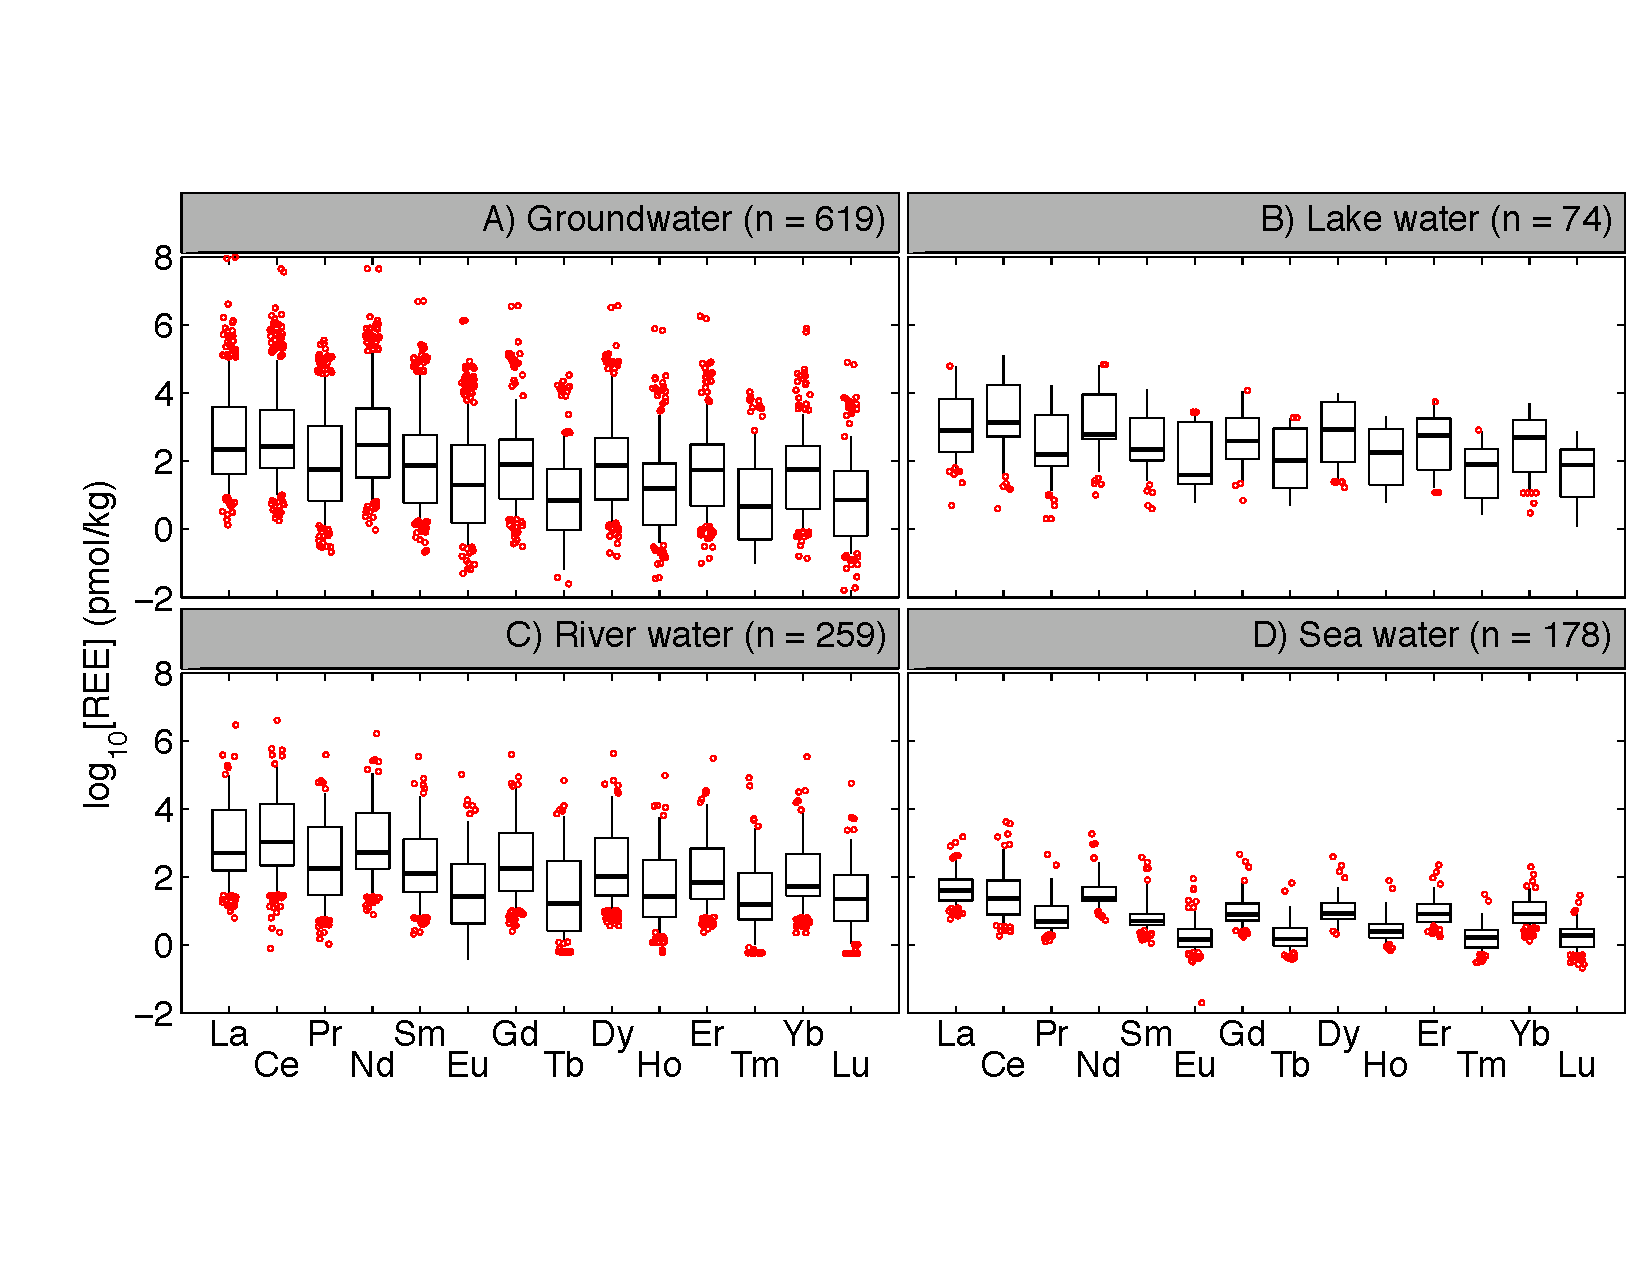
\includegraphics[width=\textwidth]{Ch3_figures/REE-water-boxplot.pdf}
\caption{REE concentration distributions in waters of different types.
Boxplots are based on source-size weighted Kaplan-Meier estimates of REE concentration percentiles and represent the median (thick, black line), inter-quartile range (IQR; first to third quartile; boxed range), 5th to 95th percentile range (whiskers), and remaining outliers (red circles).
In each subfigure heading, ``n'' in the parenthesis denotes the total number of measurements in each water type The number of detected measurements varies between elements.
These data are inclusive, representing unique water sources, spatial and temporal variations within an individual water, and any duplicate analyses.}\label{fig:all_waters}
\end{center}
\end{figure}

\begin{figure}[htbp]
\begin{center}
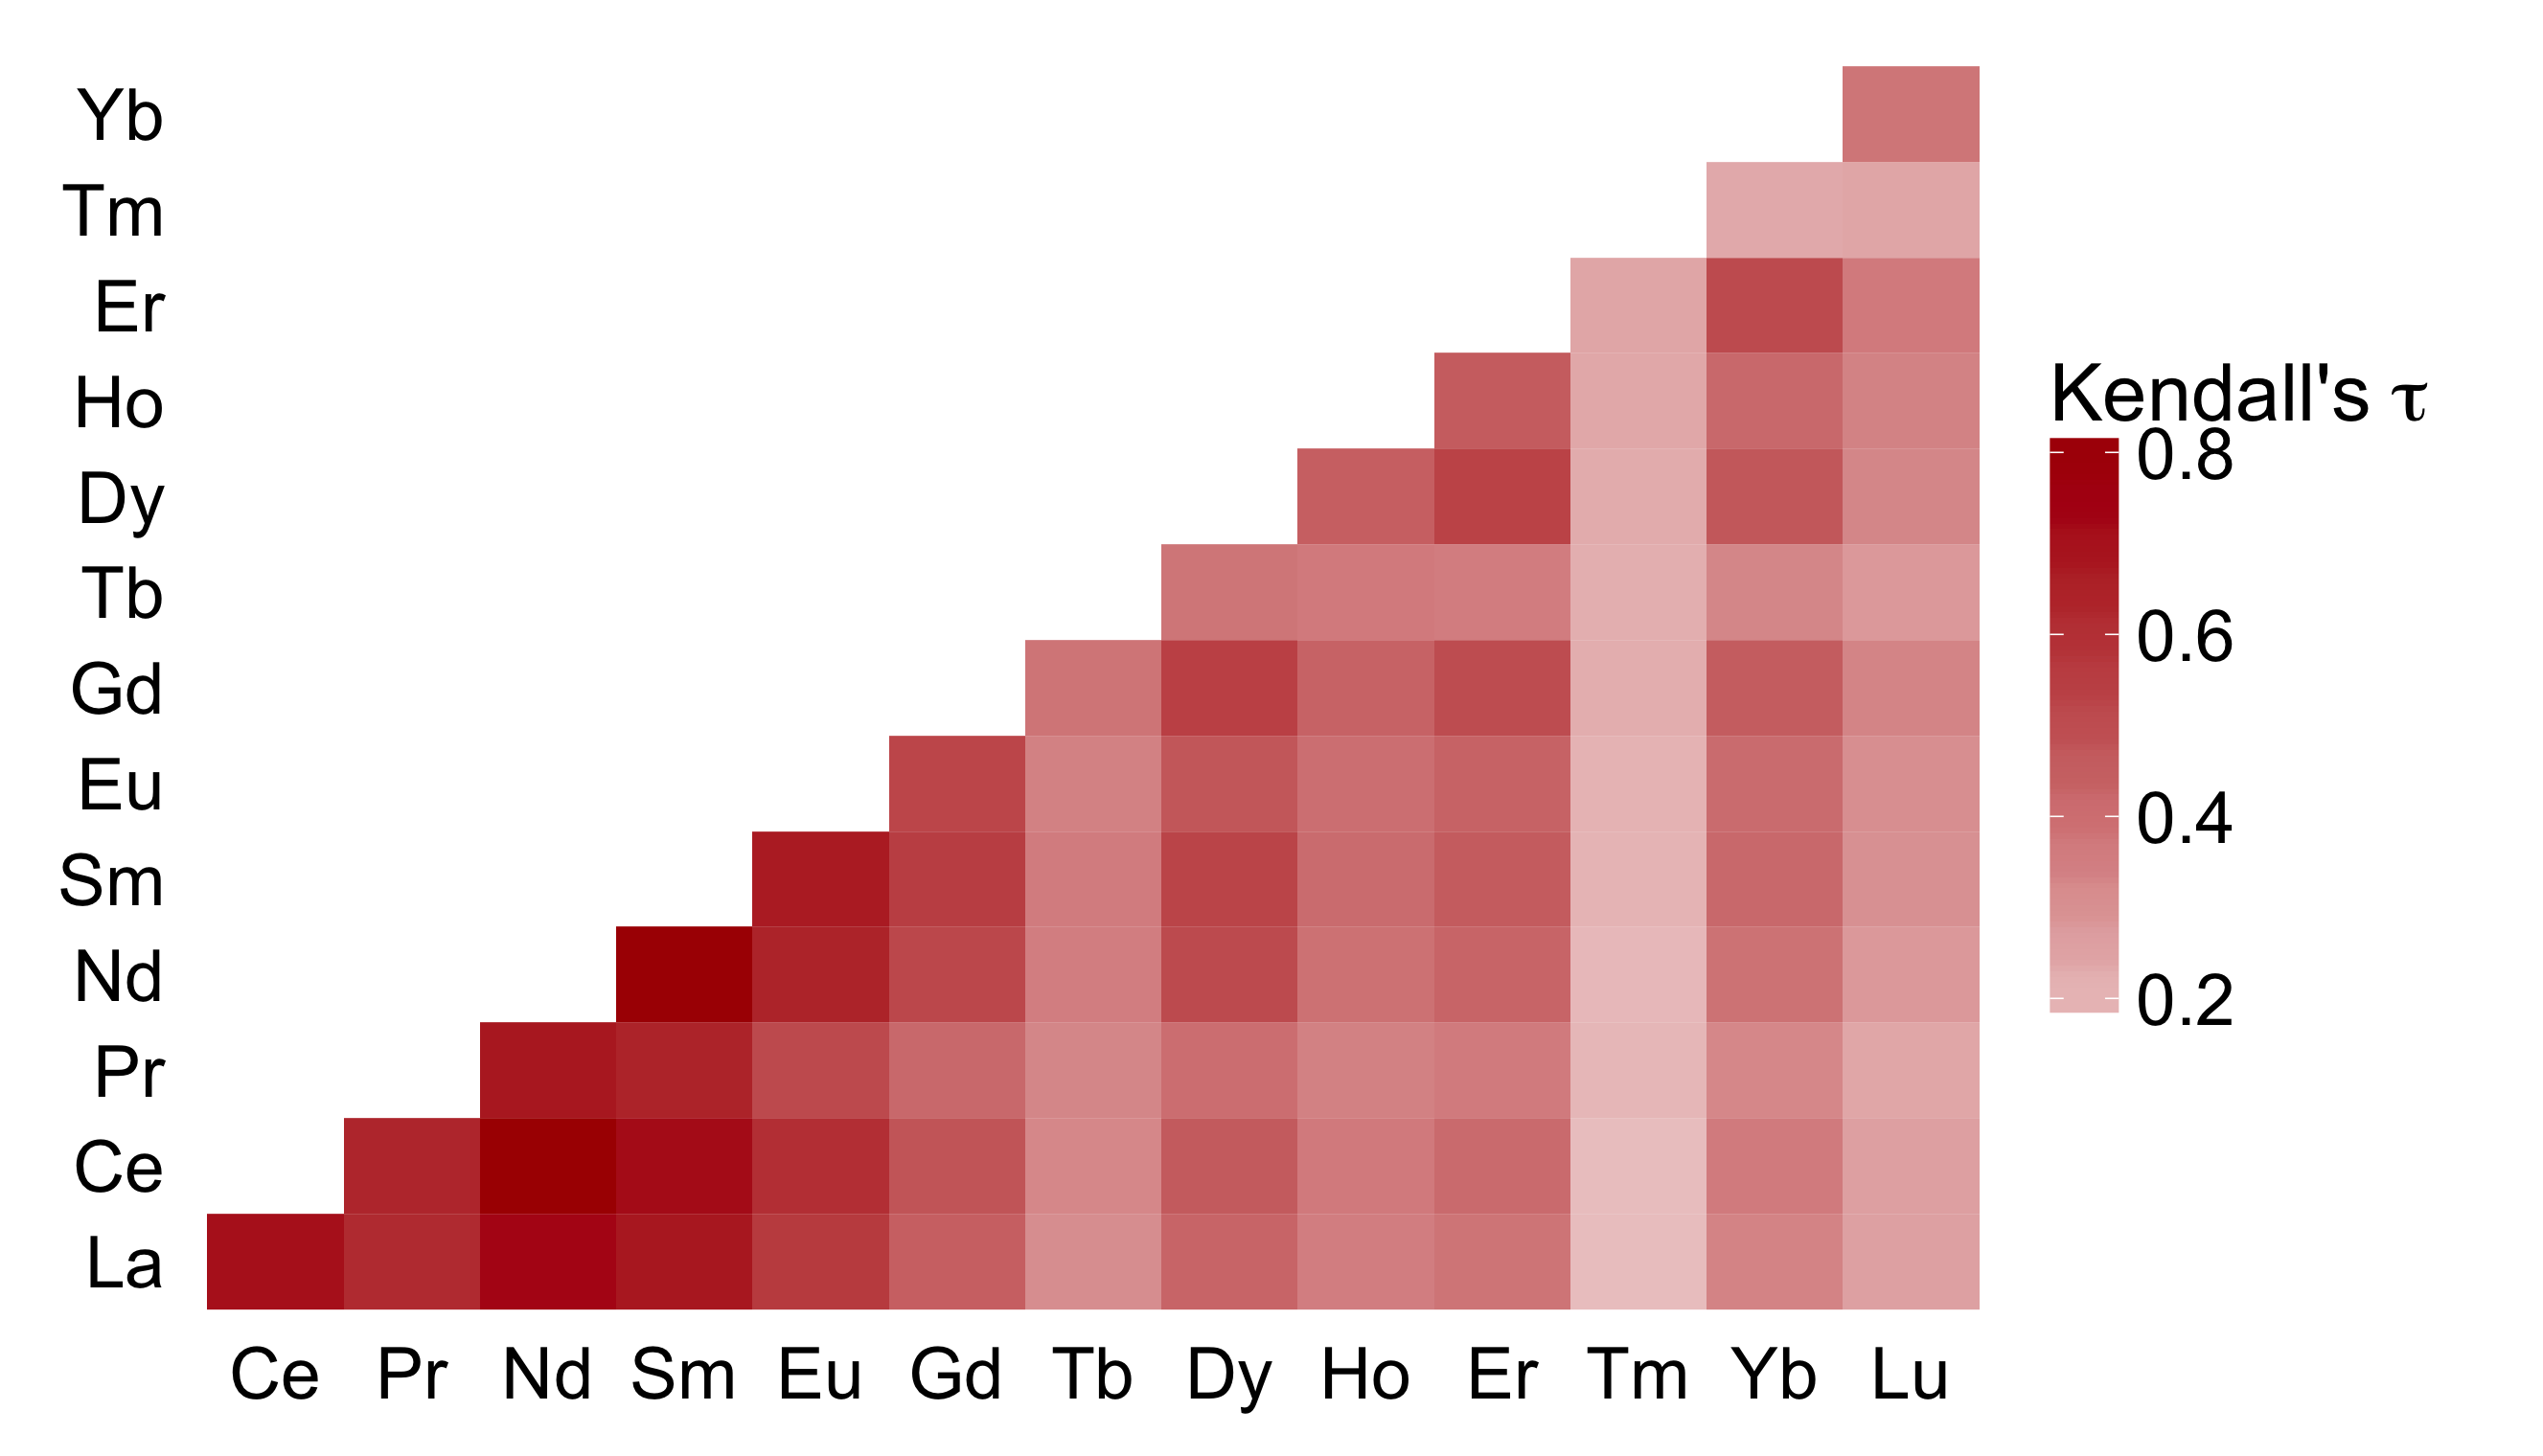
\includegraphics[width=\textwidth]{Ch3_figures/GW-ken-tau.png}
\caption{Heatmap visualization of Kendall's $\tau$ correlation coefficients among the REE in the groundwater dataset.
All correlations are statistically significantly positive.}\label{fig:REE_ken}
\end{center}
\end{figure}

\subsubsection{Groundwater}

In groundwater, the KM-calculated interquartile ranges (KM-IQR, first and third quartile) of overall REE concentrations vary between 5.7 and 410 pmol/kg solution (pmol/kg; Figure~\ref{fig:all_waters}A).
The mean concentration of the groundwater dataset was $3.5 \times 10^4$ pmol/kg and the median was 53 pmol/kg.
As shown in the disparity between the mean and median, REE concentrations in groundwater were heavily right-tailed with many ``outlier'' values and a maximum of $9.7 \times 10^6$ pmol/kg \citep{Miekeley_JGE_1992}.
The REE profile of a groundwater is thought to arise either from water-rock interactions \citep{Willis_CG_2011, Smedley_GCA_1991}
or by changes in the aqueous chemistry \citep{Dia_GCA_2000},
e.g., in relation to the residence time within the aquifer \citep{Johannesson_GW_1997, BwireOjiambo_AG_2003}.

By comparison, substitution of censored data between 0 and 100\% of the detection limit values (without source weighting) results in medians ranging from 4.4 to 13 pmol/kg and mean values ranging from $4.7 \times 10^4$ to $4.9\times 10^4$ pmol/kg.
Alternatively, deletion of below detection data roughly doubles all KM summary statistic estimates: 120 and $5.3\times 10^4$ pmol/kg for median and mean respectively.
Linear interpolation to fill in censored data also leads to significant error (Figure~\ref{fig:interp_error}).
This highlights the criticality of applying appropriate tools in calculating relevant summary statistics, particularly for quantitative analysis.

\begin{figure}[htbp]
\begin{center}
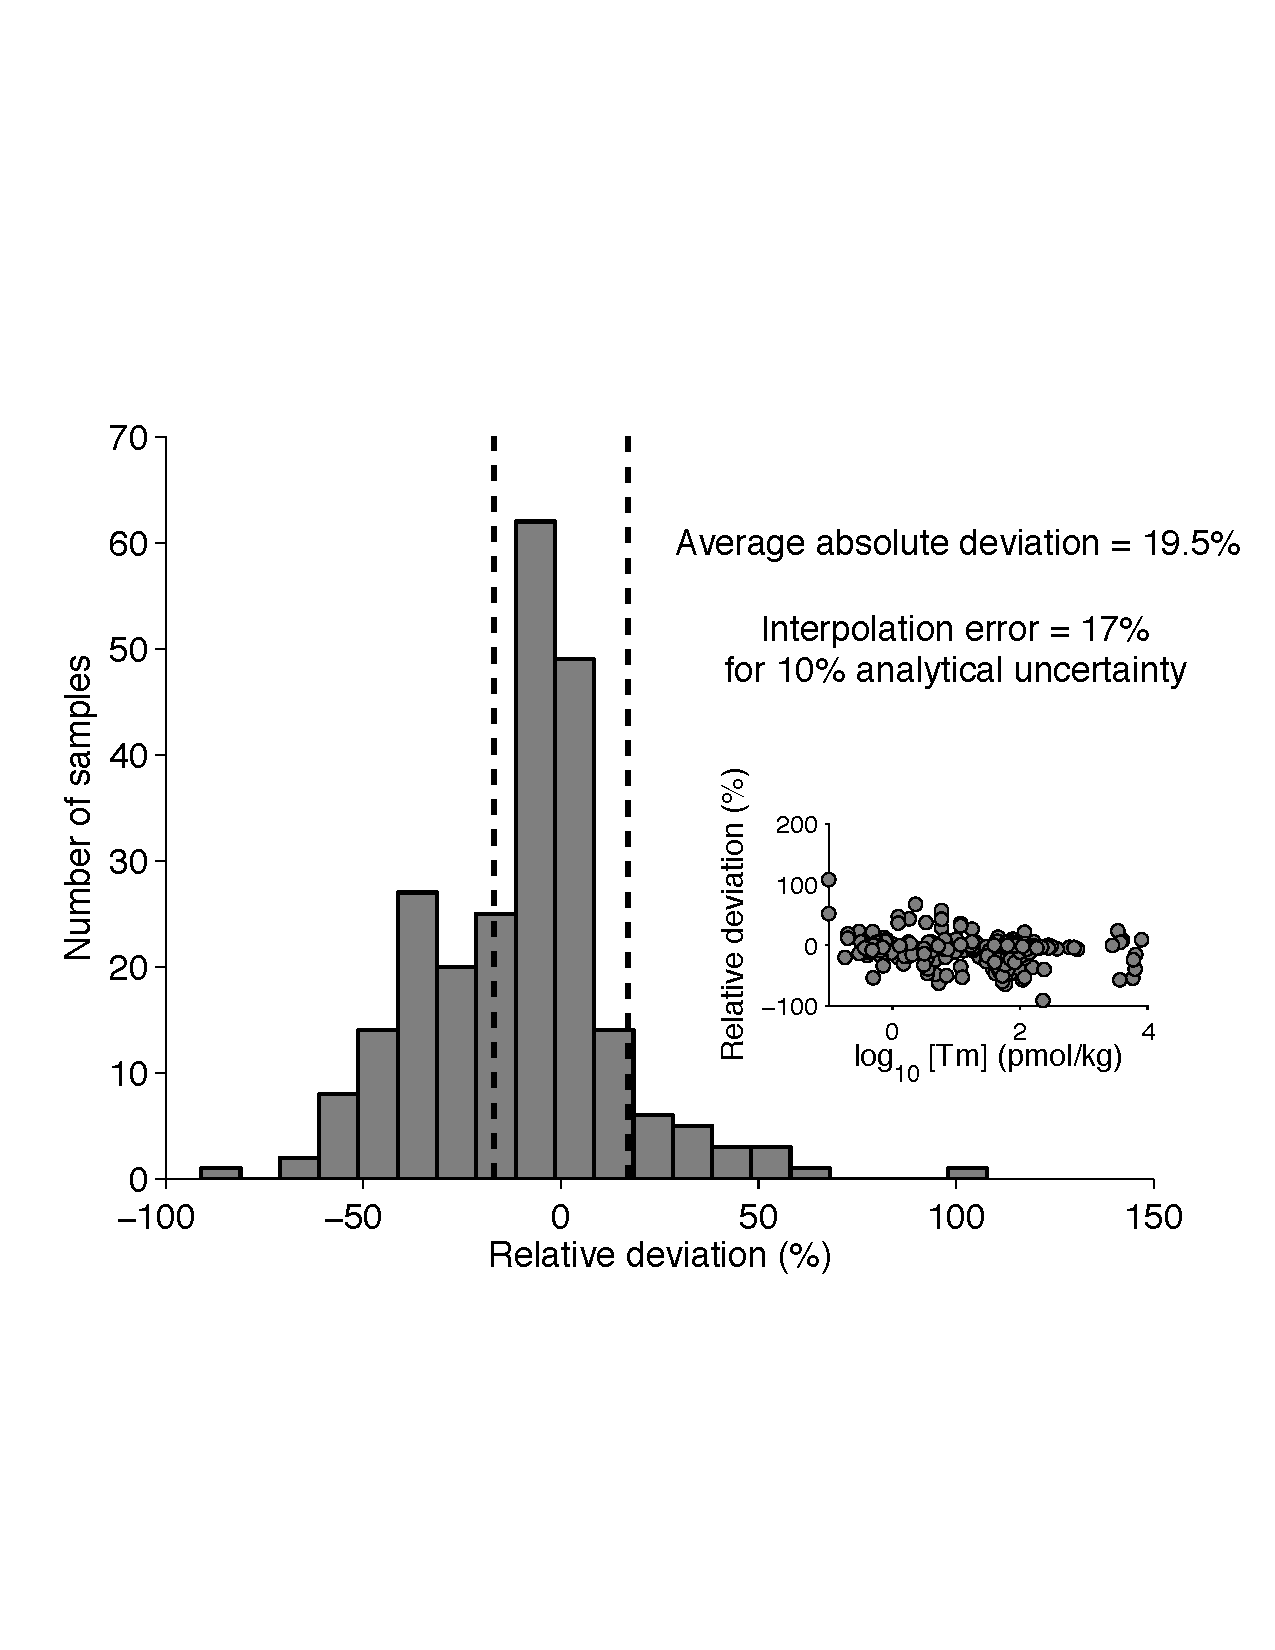
\includegraphics[width=0.8\textwidth]{Ch3_figures/Tm-interpolation-error.pdf}
\caption{Histogram of relative Post Archaean Averaged Shale normalized interpolation error of Tm in groundwater dataset and (inset) dependence of error on measured Tm values.
PAAS normalized Er and Yb were used to ``guess'' the Tm concentration and then compared to the actual measured Tm concentrations. Dashed lines mark the bounds of 10\% analytical uncertainty propagated through the interpolation.
In this analysis 42\% of 241 samples exhibit interpolation error outside the bounds of analytical uncertainty. }\label{fig:interp_error}
\end{center}
\end{figure}

\subsubsection{Terrestrial surface water}

In lake water, the KM-IQR of overall REE concentrations varied between 30 and $1.4\times10^3$ pmol/kg (Figure~\ref{fig:all_waters}B).
The mean concentration of the lake water dataset was $3.8\times10^3$ pmol/kg and the median was 170 pmol/kg.

In river water, the KM-IQRs of overall REE concentrations varied between 15 and 270 pmol/kg (Figure~\ref{fig:all_waters}C).
The mean concentration of the river water dataset was $3.3\times10^3$ pmol/kg and the median was 71 pmol/kg.

\subsubsection{Seawater}

In seawater, the KM-IQR of reported REE concentrations varied between 1.6 and 13 pmol/kg (Figure~\ref{fig:all_waters}D).
The mean concentration of the seawater dataset was 19 pmol/kg and the median was 5 pmol/kg.
The disparity between the dissolved REE in seawater and its influent waters is likely attributable to particulate scavenging \citep{Sholkovitz_GCA_1994, Erel_GCA_1993} at a rate that exceeds mass fluxes from surface- and groundwater sources.
In groundwater by comparison, continuous weathering of the aquifer rock counteracts sorption and co-precipitation loss mechanisms.
Dubinin \citep{Dubinin_LMR_2004} notes that dissolved fractions of REE increase with distance off-shore as terrigenous material settles, which removes REE mass faster than it can be replenished by other sources such as aeolian deposition or hydrothermal venting

\subsubsection{Shale-normalized anomalies and ratios}

The groundwaters in this dataset primarily exhibited mild negative and positive shale-normalized anomalies for Ce and Eu respectively, though, as with abundance, these RDVs varied widely (Figure~\ref{fig:all_RDV}).
Both terrestrial surface waters reported here exhibit similar Ce* and Eu* (Figure~\ref{fig:all_RDV}A and~\ref{fig:all_RDV}B), which are mildly negative and nearly zero respectively.
The Ce* of seawater is starkly different that any of the three water types, developing consistent, negative anomalies with instances of large positive anomalies. 

Nearly all waters in this study are LREE depleted (Figure~\ref{fig:all_RDV}C and~\ref{fig:all_RDV}D).
As with element anomalies, the mean and IQR of interelement ratios among groundwaters and terrestrial surface waters are similar while seawater exhibits distinctly lower ratios.
Both anomalies in groundwater exhibit large outlier values, similar to REE abundance, which underscores the extreme variability in groundwater systems.

\begin{figure}[htbp]
\begin{center}
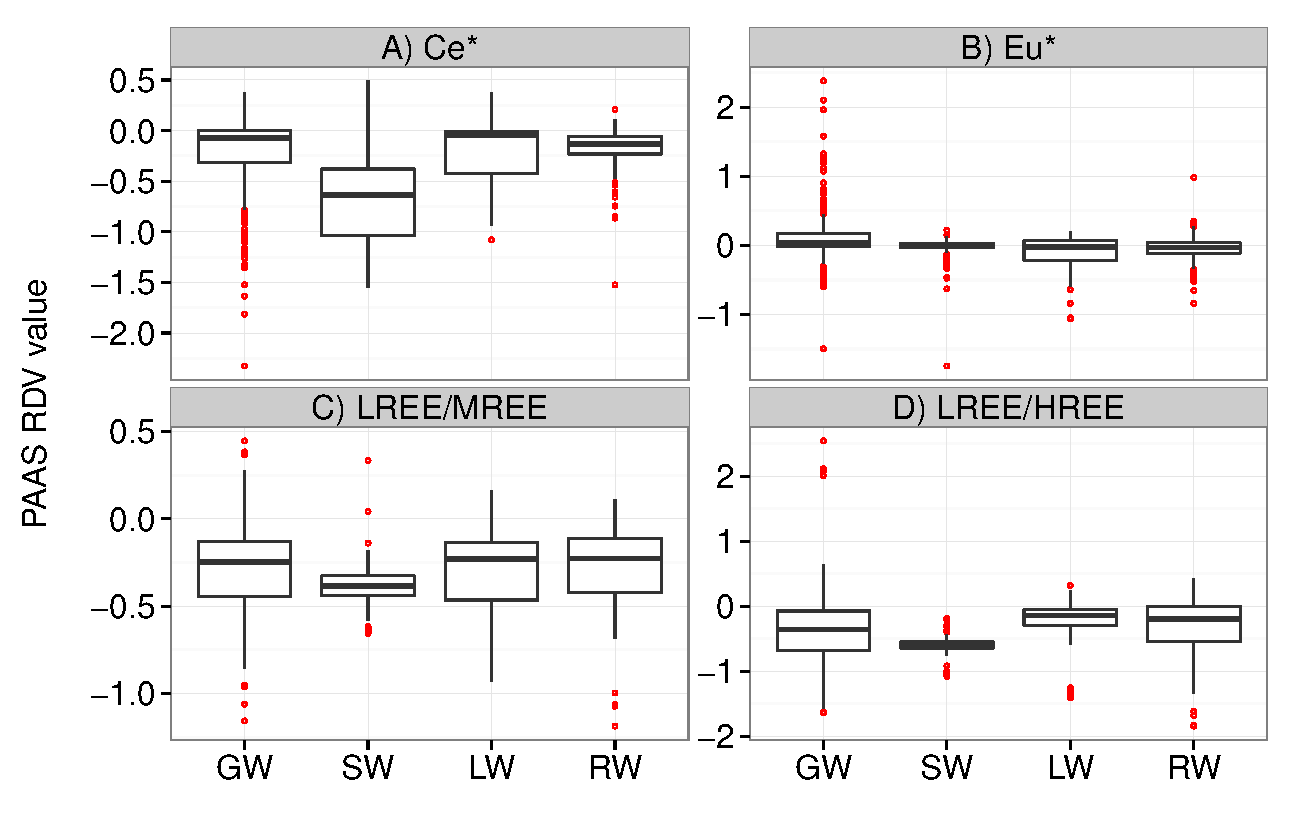
\includegraphics[width=0.8\textwidth]{Ch3_figures/REE-waters-RDV-boxplots.pdf}
\caption{Log-transformed, Post-Archaean Average Shale (PAAS)- normalized, reduced dimension variables (RDVs) calculated for groundwater (GW), seawater (SW), lake water (LW), and river water (RW) data.
RDVs are the cerium anomaly (Ce*), europium anomaly (Eu*), LREE / MREE ratio, and LREE / HREE ratio.
Boxplots represent the median (thick, black line), interquartile range (IQR; first to third quartile; boxed range), $\pm1.5$ times the IQR (whiskers), and remaining outliers (red circles).}\label{fig:all_RDV}
\end{center}
\end{figure}

The anomalies of Ce and Eu are of interest because they are the two REE with redox lability within the Eh-pH regime of water stability \citep{Brookins_GJ_1983}.
Upon oxidation -- Ce(III) to Ce(IV) -- cerium readily precipitates as \ce{CeO2}(s);
alternatively, europium becomes less soluble when reduced from Eu(III) to Eu(II) based on preferential incorporation into other minerals due to the lower valency and higher ionic radius of the reduced state (similar to Sr) \citep{Brookins_RMG_1989}.
Where anomalies in rock samples have been used to infer paleo-redox conditions, the anomalies in aqueous samples are often used to analyze water-rock interactions \citep{Willis_CG_2011, Smedley_GCA_1991}.

Divalent europium is energetically favorable under extremely reducing conditions or at high temperatures.
Reduced Eu(II) exhibits strong partitioning to various minerals during crystallization from magmatic fluids.
Thus many source rocks are either highly enriched (e.g. plagioclase \citep{Nash_GCA_1985}) or highly depleted (e.g. olivine \citep{Foley_Lithos_2004} and pyroxene \citep{Hanson_EPS_1980}) in Eu, enhancing or limiting availability during weathering \citep{Sverjensky_EPSL_1984}.
In hot, reduced, alkaline waters fracture filling calcite commonly contains notable Eu enrichments indicating that the source fluids developed negative Eu* \citep{Lee_AG_2003, Cai_AG_2008}.
However, such environments are representative of hydrothermal waters \citep{Sverjensky_EPSL_1984}, which have specifically excluded from this analysis.
Thus the Eu* in this dataset are thought to result from mineral weathering \citep{Sverjensky_EPSL_1984}.

While aquatic redox couples are commonly in disequilibrium for measured redox potential (Eh) \citep{Linberg_Sci_1984}, Figure~\ref{fig:anom_vs_Eh}A illustrates a negative correlation ($\rho=-0.33$; $P<1\times10^{-6}$) between $Ce_N^*$ and Eh in groundwater, as expected for oxidative scavenging.
However, the low strength of the correlation reflects the mechanism being a function of both source composition and aqueous chemistry.
Europium anomalies do not exhibit the expected positive trend with redox potential in groundwater, though a weak negative correlation is observed ($\rho= -0.18$, $P = 0.006$; Figure~\ref{fig:anom_vs_Eh}B).
Stability diagrams with measure Ce* and Eu* are included in Figure~\ref{fig:pourbaix} and show the lack of agreement between measured and thermodynamically predicted anomalies.

\begin{figure}[htbp]
\begin{center}
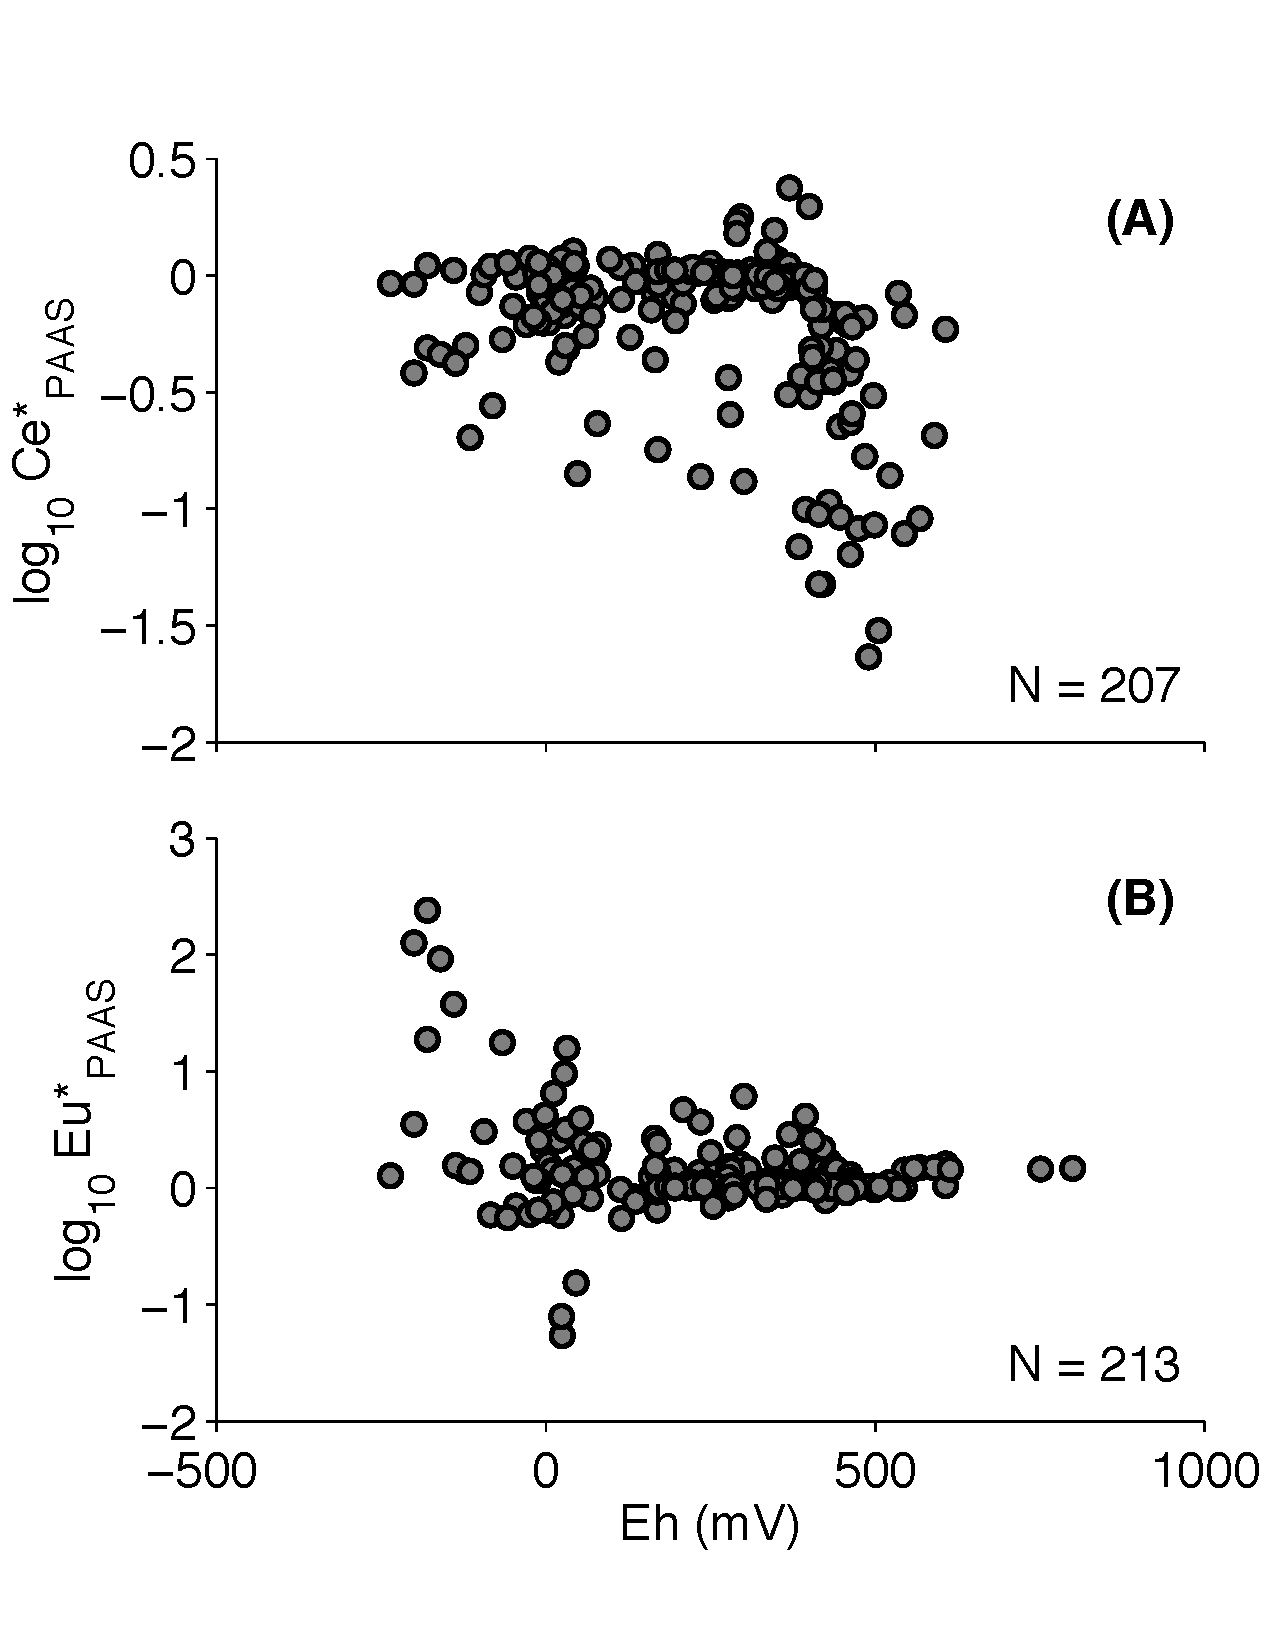
\includegraphics[width=0.5\textwidth]{Ch3_figures/Ce-Eu-anom-vs-Eh.pdf}
\caption{Groundwater Post-Archaean Average Shale (PAAS) Ce anomaly (Ce*, A, Eq.~\ref{eq:CeAnom}) and Eu anomaly (Eu*, B) as a function of reported redox potential (Eh).
Sample size denoted by ``N''.}\label{fig:anom_vs_Eh}
\end{center}
\end{figure}

\begin{figure}[htbp]
\begin{center}
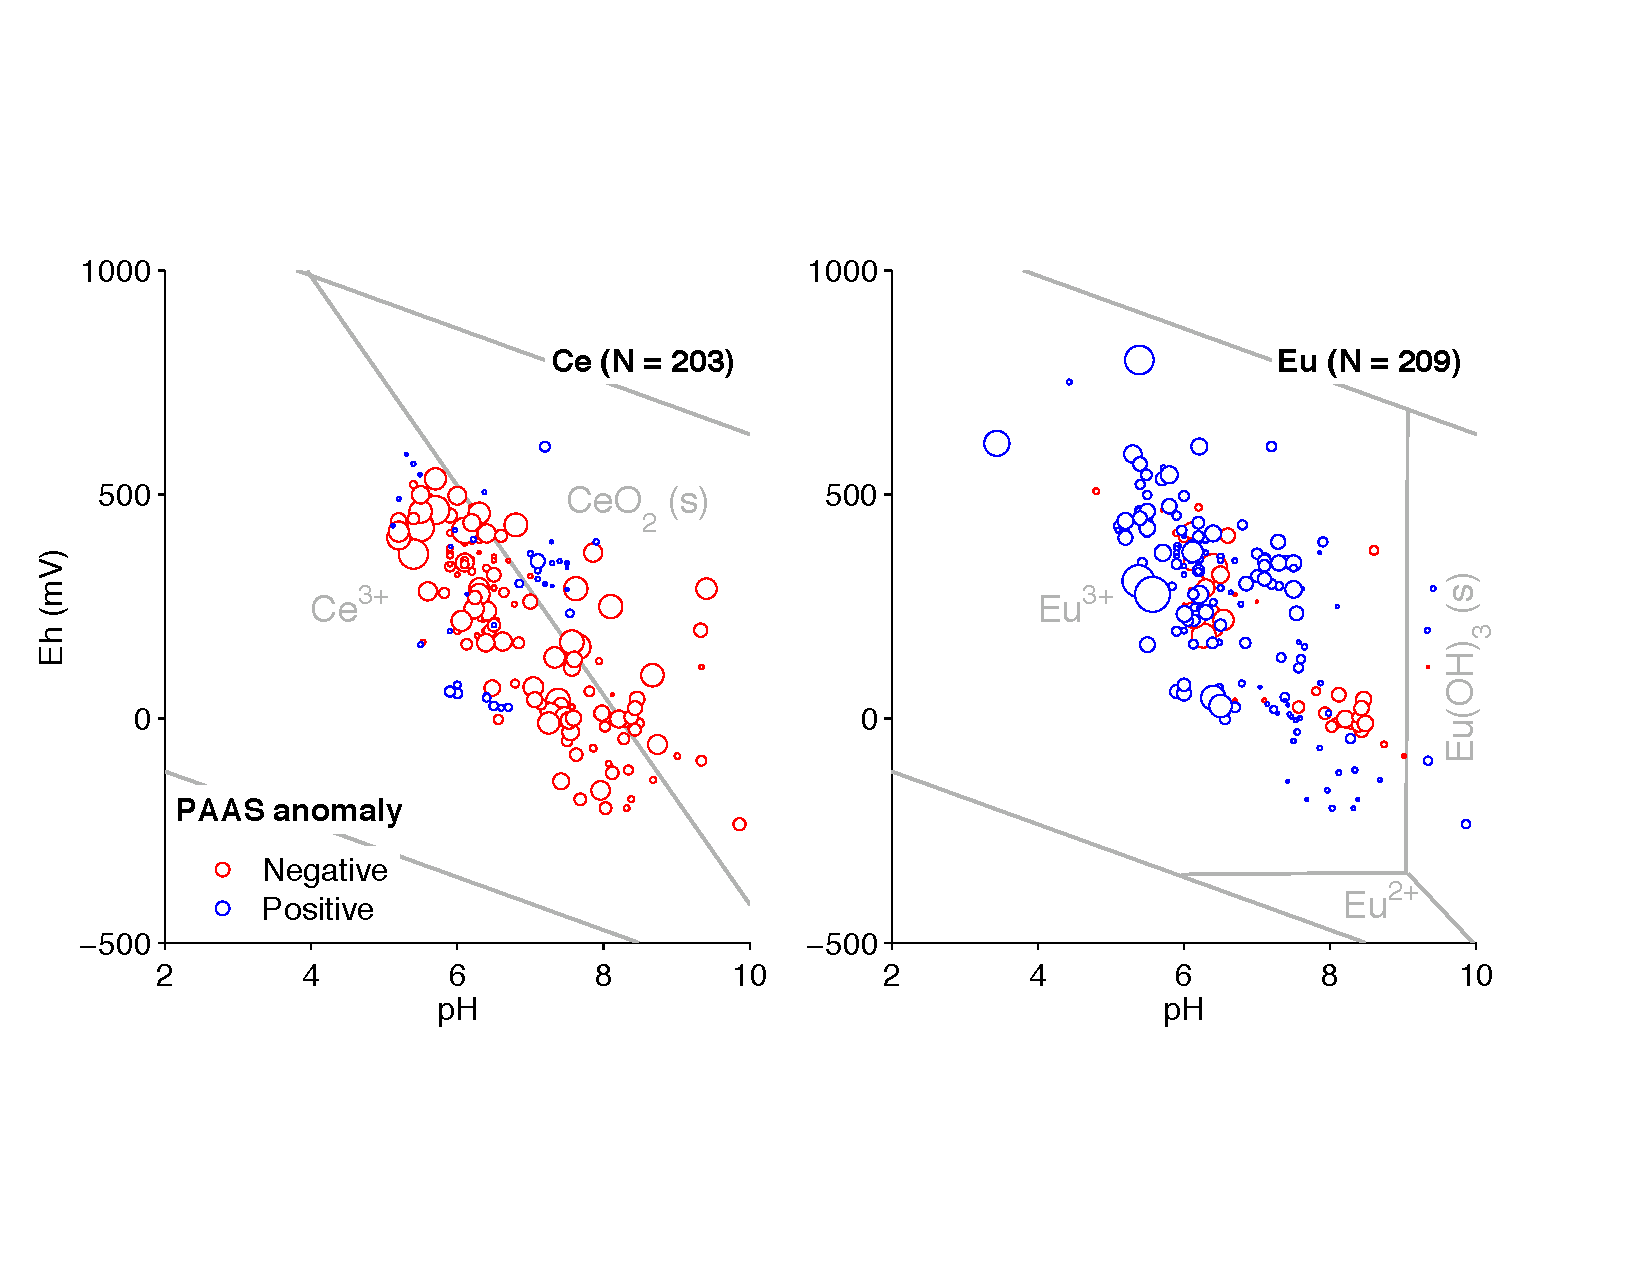
\includegraphics[width=\textwidth]{Ch3_figures/Ce-Eu-stability-anom.pdf}
\caption{Post-Archaean Average Shale (PAAS) Cerium (Ce; left) and Europium (Eu; right) anomalies as functions of redox potential (Eh) and pH.
Marker color corresponds to the sign of the anomaly and marker size corresponds to the magnitude of the anomaly.
Stability fields, reproduced from Brookins \citep{Brookins_RMG_1989}, for relevant species in the REE-\ce{H2O} system underlie the data for TOTCe$=$TOTEu $=10^{-11}$ M at 298 K}\label{fig:pourbaix}
\end{center}
\end{figure}

\subsection{REE abundance trends in groundwater}

Of all the bulk solution chemistry parameters for groundwater, pH exerted the greatest control as an independent variable over dissolved REE abundance (Figure~\ref{fig:sum_vs_pH}). Generally, more acidic waters contained the most REE, either via acidification-enhanced weathering or from an enrichment of REE in the acid source \citep{Dia_GCA_2000, Smedley_GCA_1991, Gosselin_GCA_1992, Janssen_WR_2003, Worrall_AG_2001, Leybourne_AG_2000, Miekeley_JGE_1992}.
REE are effectively scavenged from more neutral and basic waters via sorption onto oxides and clays or co-precipitation with carbonates and phosphates by replacing calcium, which has a comparable atomic radius \citep{Johannesson_LO_1994, CRC_handbook, Bradbury_GCA_2002, Coppin_CG_2002, Quinn_MC_2006, Terakado_CG_1988}.
Over the pH range 4-8, dissolved REE abundance follows an approximate $-1$ slope with increasing pH (95\% confidence interval of $-1.02 \pm 0.1$), indicative of a single-proton (i.e. mono-dentate) surface complexation reaction or calcite precipitation when carbonate far exceeds calcium \citep{Morel_Herring}.
Geochemical modeling showed that nearly all samples were significantly undersaturated with respect to either pure-phase REE hydroxides or carbonates (Figure~\ref{fig:REE_SI}).

\begin{figure}[htbp]
\begin{center}
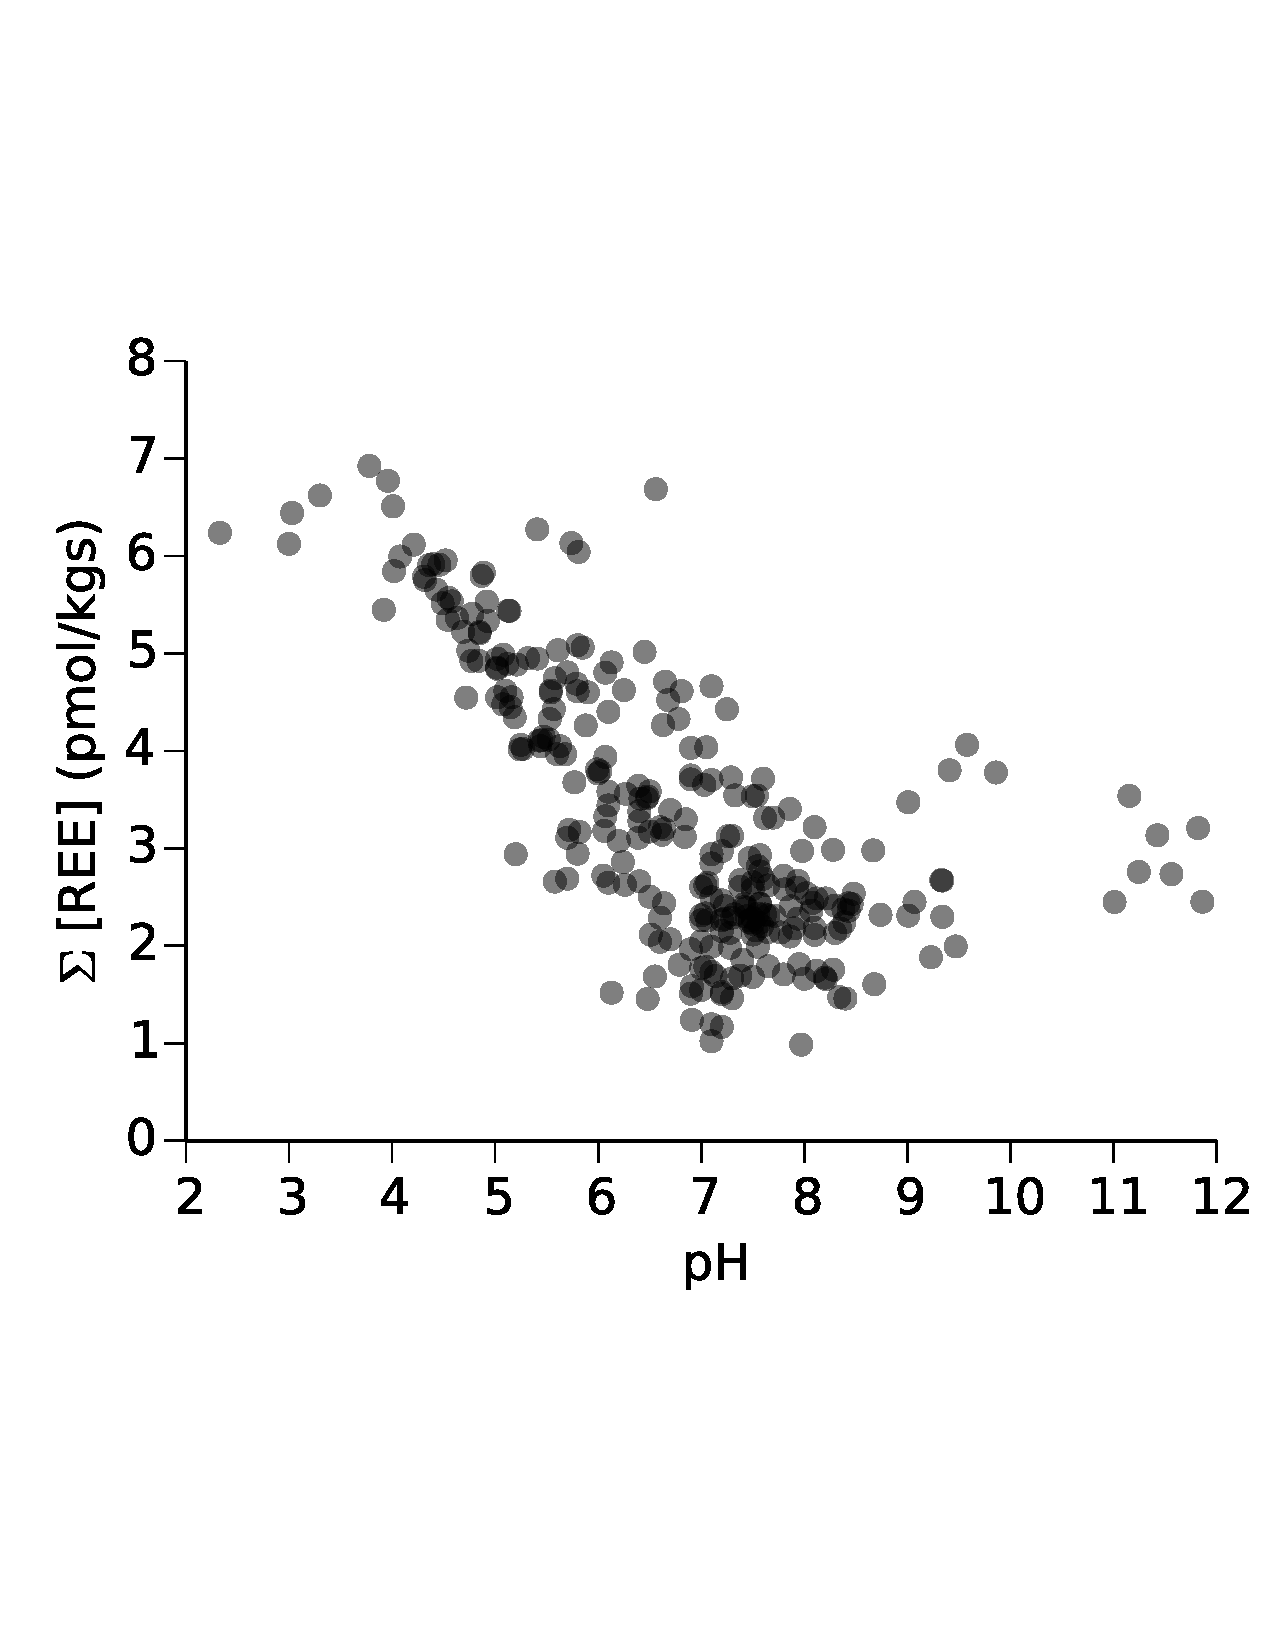
\includegraphics[width=0.67\textwidth]{Ch3_figures/tot_REE-vs-pH.pdf}
\caption{Sum of dissolved REE vs pH for groundwater data from Kaplan-Meier estimates (Eq~\ref{eq:totalREE}).
Markers are semitransparent to illustrate data density.
Data presented for 281 samples.}\label{fig:sum_vs_pH}
\end{center}
\end{figure}

\begin{figure}[htbp]
\begin{center}
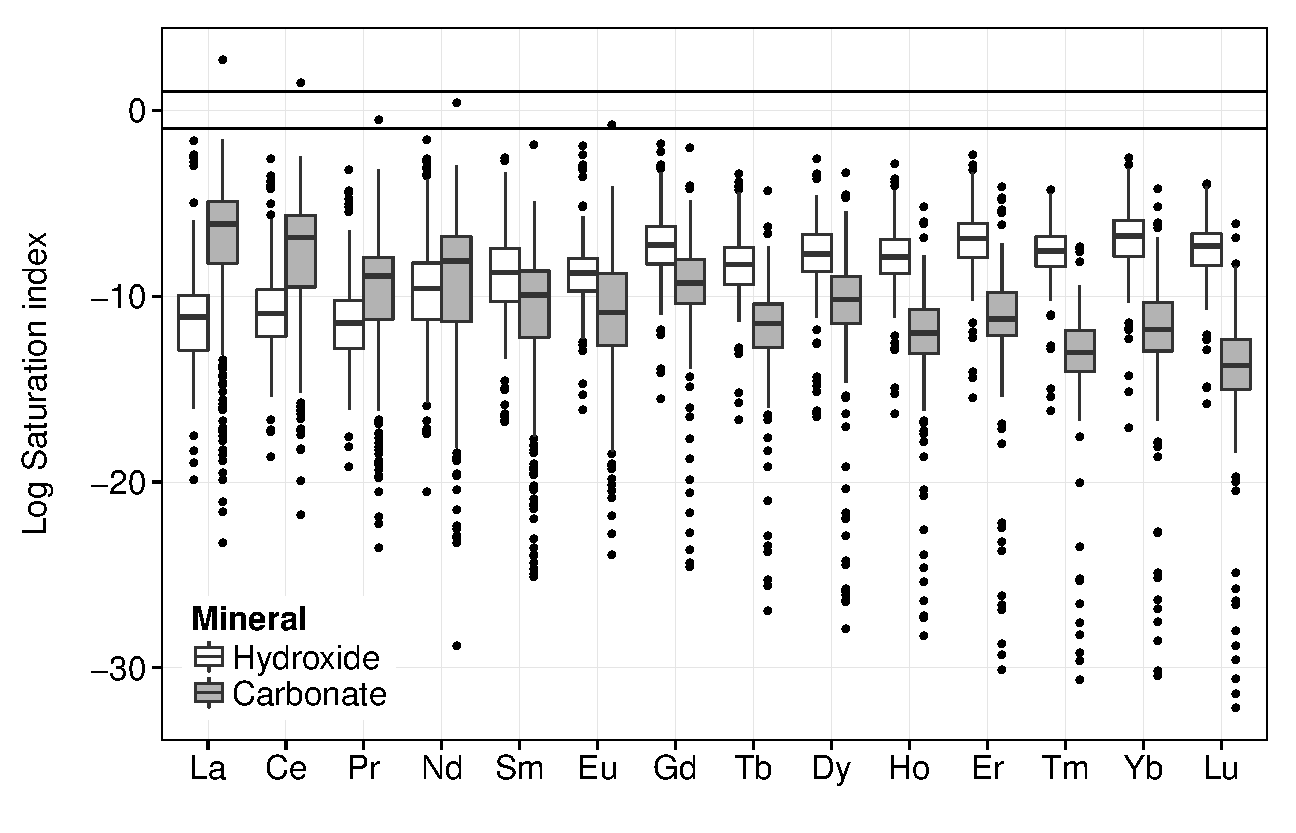
\includegraphics[width=0.8\textwidth]{Ch3_figures/REE-mineral-SI.pdf}
\caption{Modeled, log-transformed saturation indices of pure phase REE hydroxides and carbonates for groundwater data. Saturation indices calculated using PHREEQC and the LLNL database. Solid lines at $-1$ and 1 indicate range of potentially solubility controlling phases \citep{Meima_EST_1997}.}\label{fig:REE_SI}
\end{center}
\end{figure}

Strong complexation with carbonate, particularly as a dicarbonato complex (\ce{REE(CO3)2-}) is thought to account for the apparent amphoteric behavior as pH becomes more  \citep{Millero_GCA_1992, Wood_CG_1990, Johannesson_AG_1995}.
The REE form progressively stronger carbonate and dicarbonato complexes with increasing atomic number \citep{Millero_GCA_1992, Wood_CG_1990}, which would suggest an increase of MREE or HREE relative to LREE as a function of pH or carbonate ion activity.
However, such a trend is not observed within the current dataset (Figure~\ref{fig:frac_vs_acarb}) though the breadth of the current dataset may simply obscure such trends seen in individual studies \citep[e.g. Ref.][]{Choi_CG_2009}.

\begin{figure}[htbp]
\begin{center}
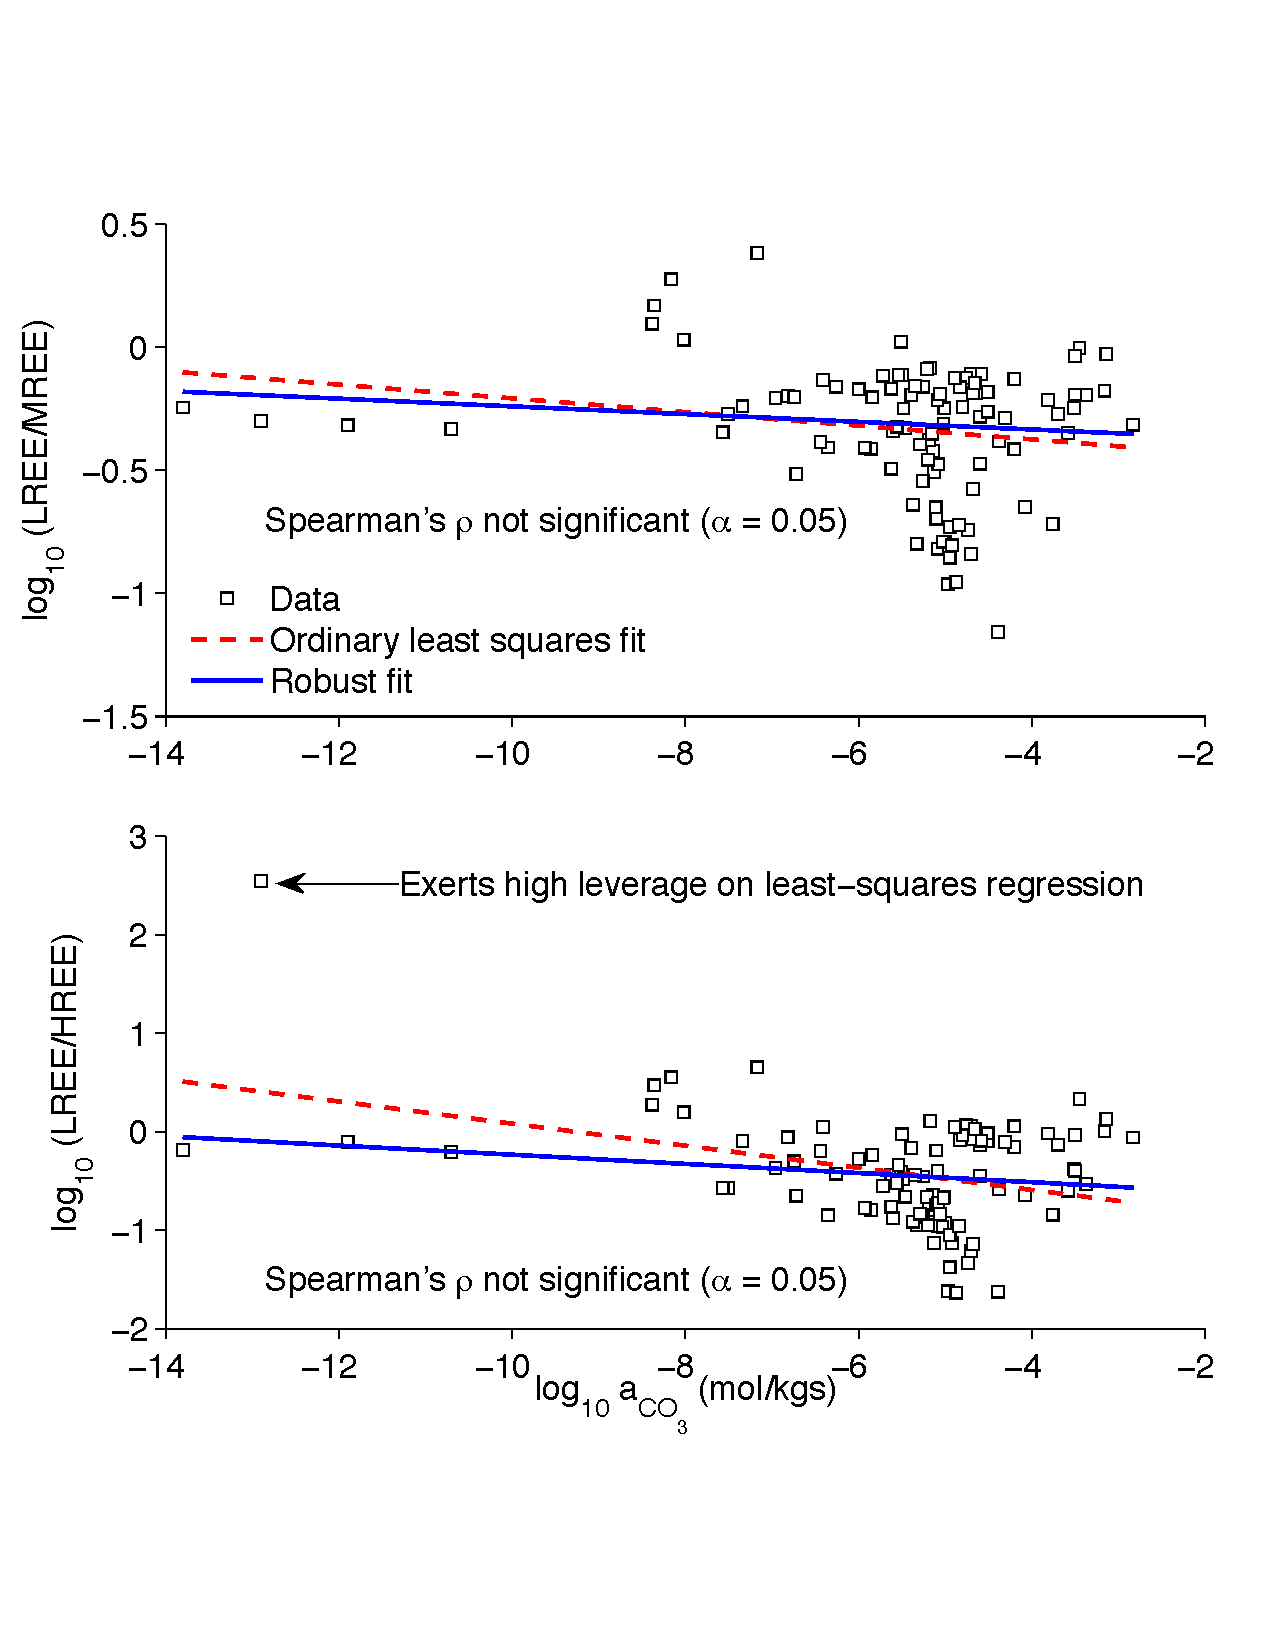
\includegraphics[width=0.8\textwidth]{Ch3_figures/REE-ratios-vs-act_carb.pdf}
\caption{Light-middle REE fractionation (top) and light-heavy REE fractionation (bottom) as a function of modeled carbonate ion activity (a$_{\ce{CO3}}$).
For L/M fractionation neither regression is significant, while L/H ordinary least squares regression is significant due to a high outlier value. Each plot contains 99 data points.}\label{fig:frac_vs_acarb}
\end{center}
\end{figure}

Kendall's $\tau$ correlation analysis of REE with bulk solutes shows inconsistent trends, however most of the meaningful relationships are between the solutes and the LREE and are weakly negative (Figure~\ref{fig:REE-vs-major}).
This behavior is contrary to many other metals that correlate positively with dissolved solids.
This likely highlights the heterogeneity of the dataset and the importance of surface reactions in controlling dissolved REE abundance.

\begin{figure}[htbp]
\begin{center}
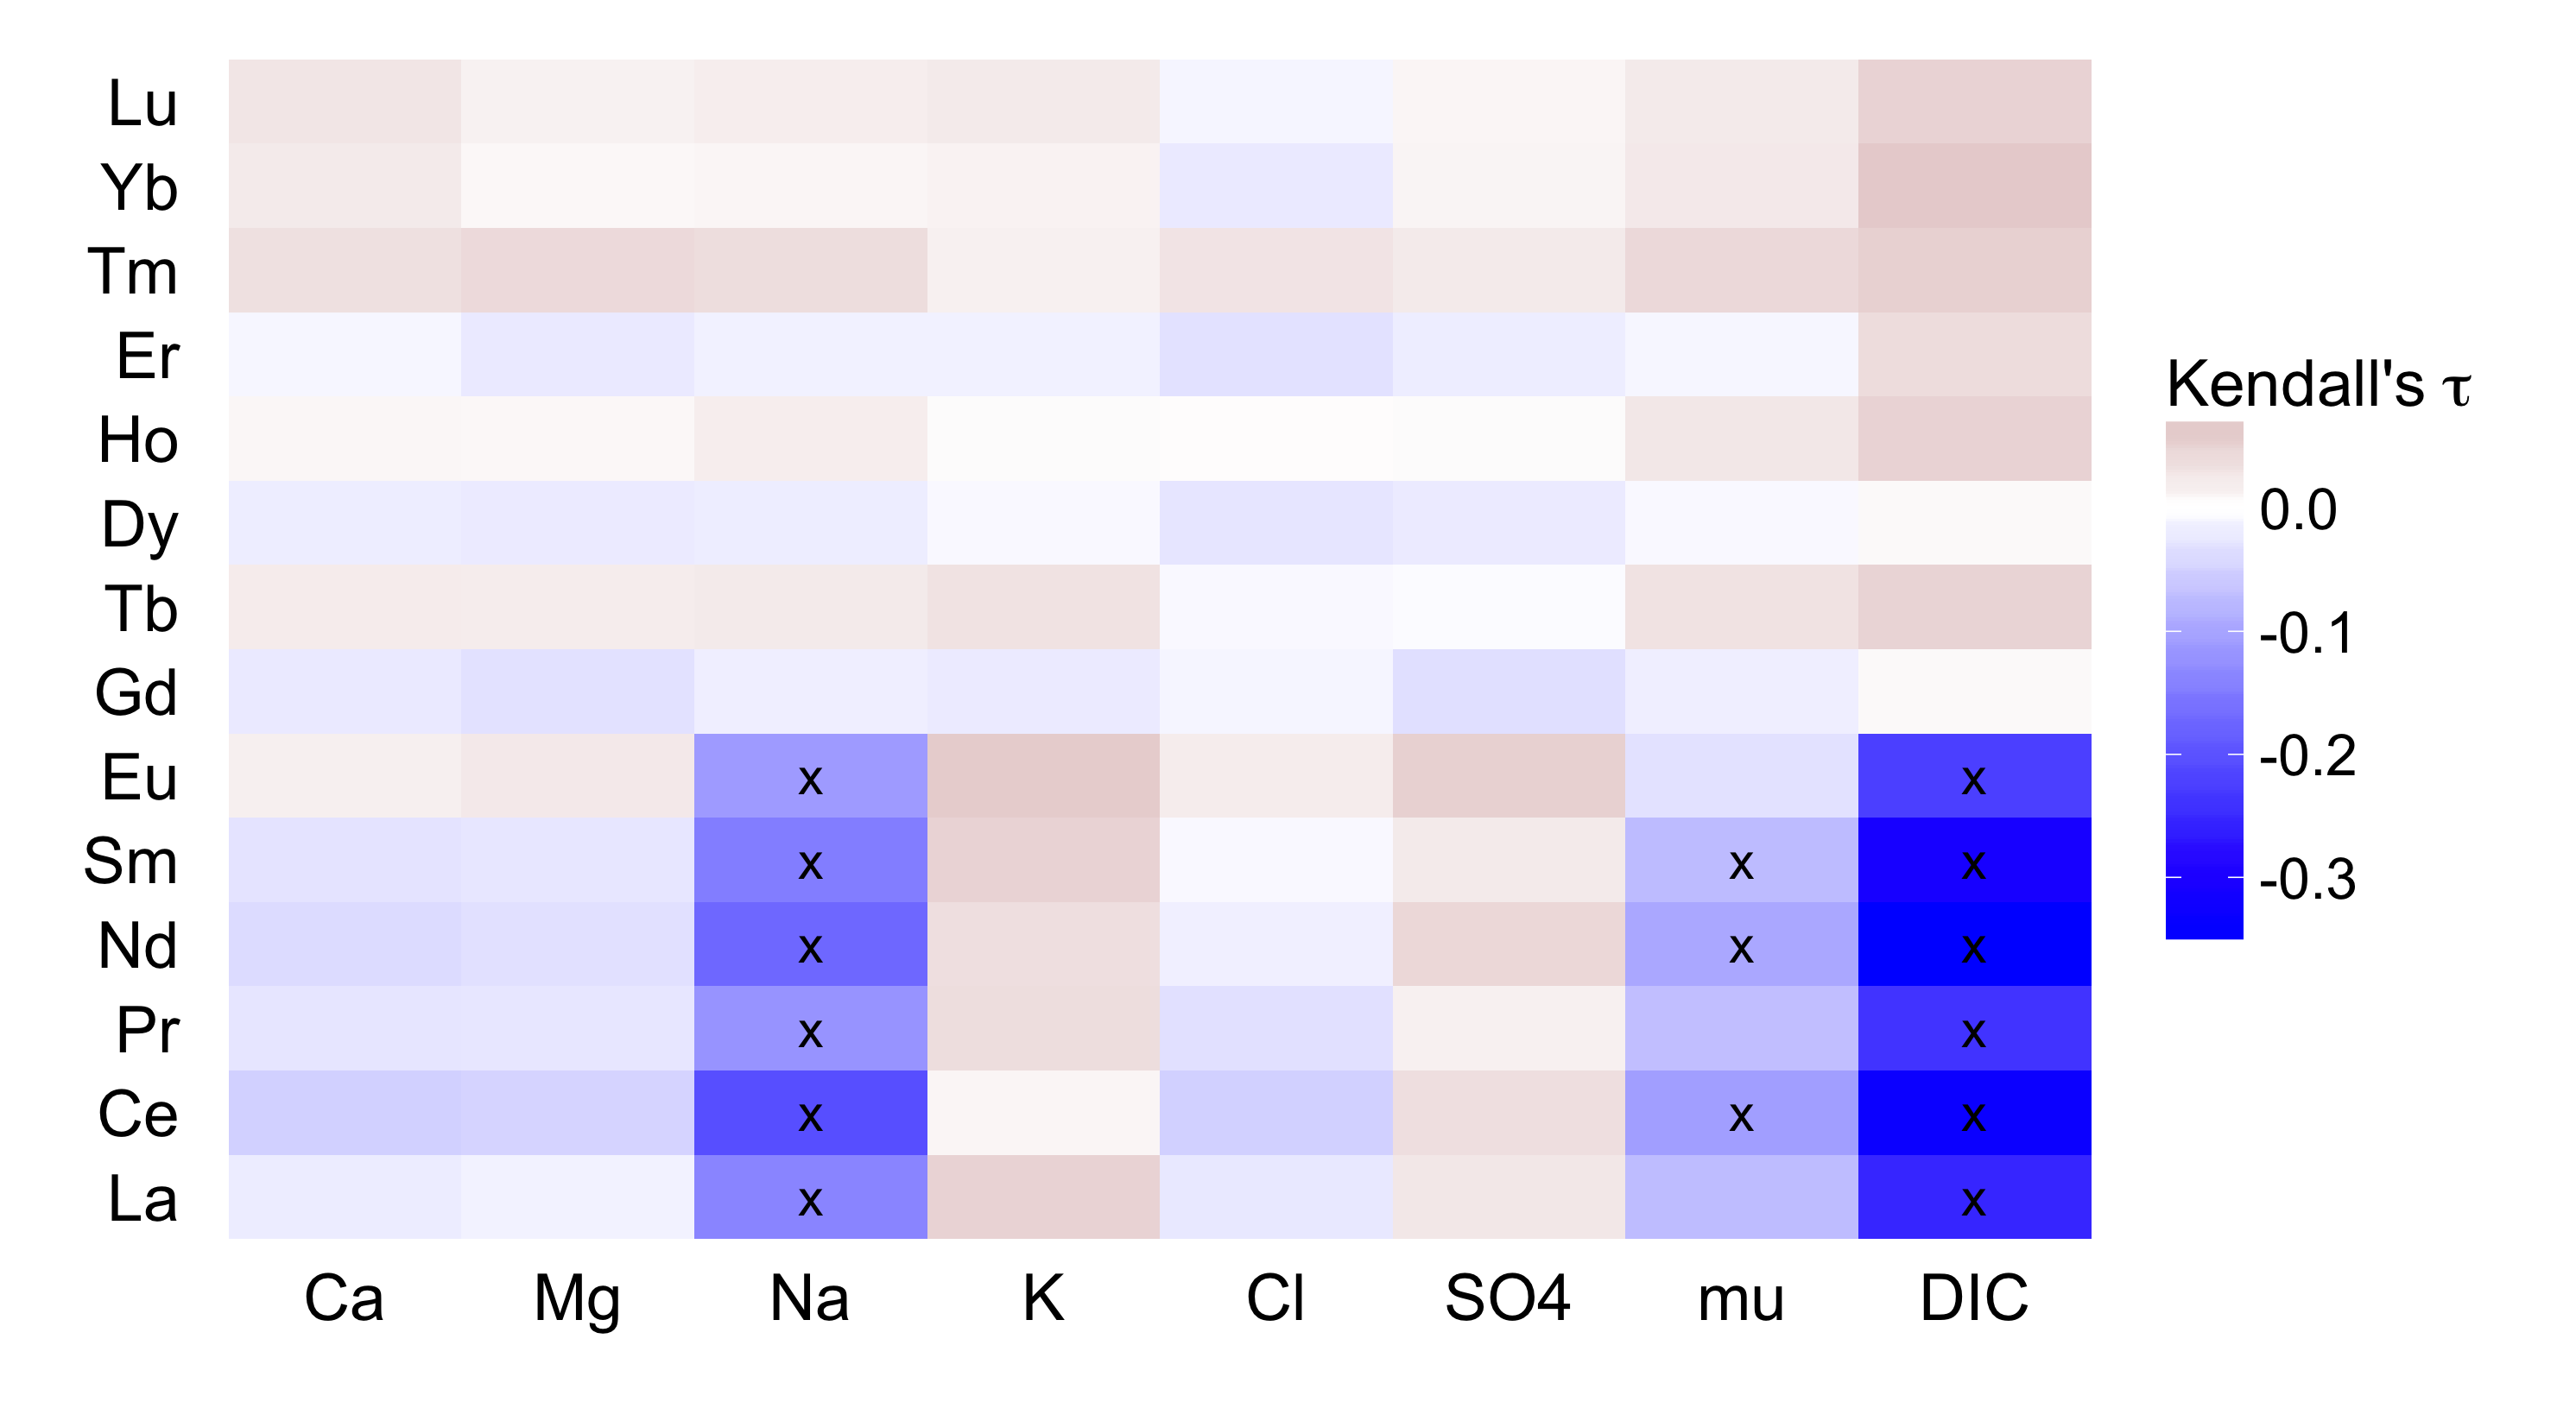
\includegraphics[width=0.9\textwidth]{Ch3_figures/REE-vs-chem.png}
\caption{Heatmap visualization  of Kendall's $\tau$ coefficients between REE abundance and total bulk solutes and calculated ionic strength (``mu'') in groundwater.
Statistically significant correlations ($\alpha = 0.05$) are noted with an ``x''.}\label{fig:REE-vs-major}
\end{center}
\end{figure}

\subsubsection{Major element chemistry of the groundwater data}

For the groundwater data, the screening process reduced the total number of samples from 619 to 328.
The representative chemistries of the screened dataset samples varied widely, with several orders of magnitude range in the major ion concentrations (Figure~\ref{fig:GW-chem-hist}).
Plotting the major ion concentrations using a Piper diagram \citep{Piper_diag} showed that the major anions were predominantly Cl/\ce{SO4}, while the predominant cations varied between monovalent and divalent (Figure~\ref{fig:GW-chem-piper}).

\begin{figure}[htbp]
\begin{center}
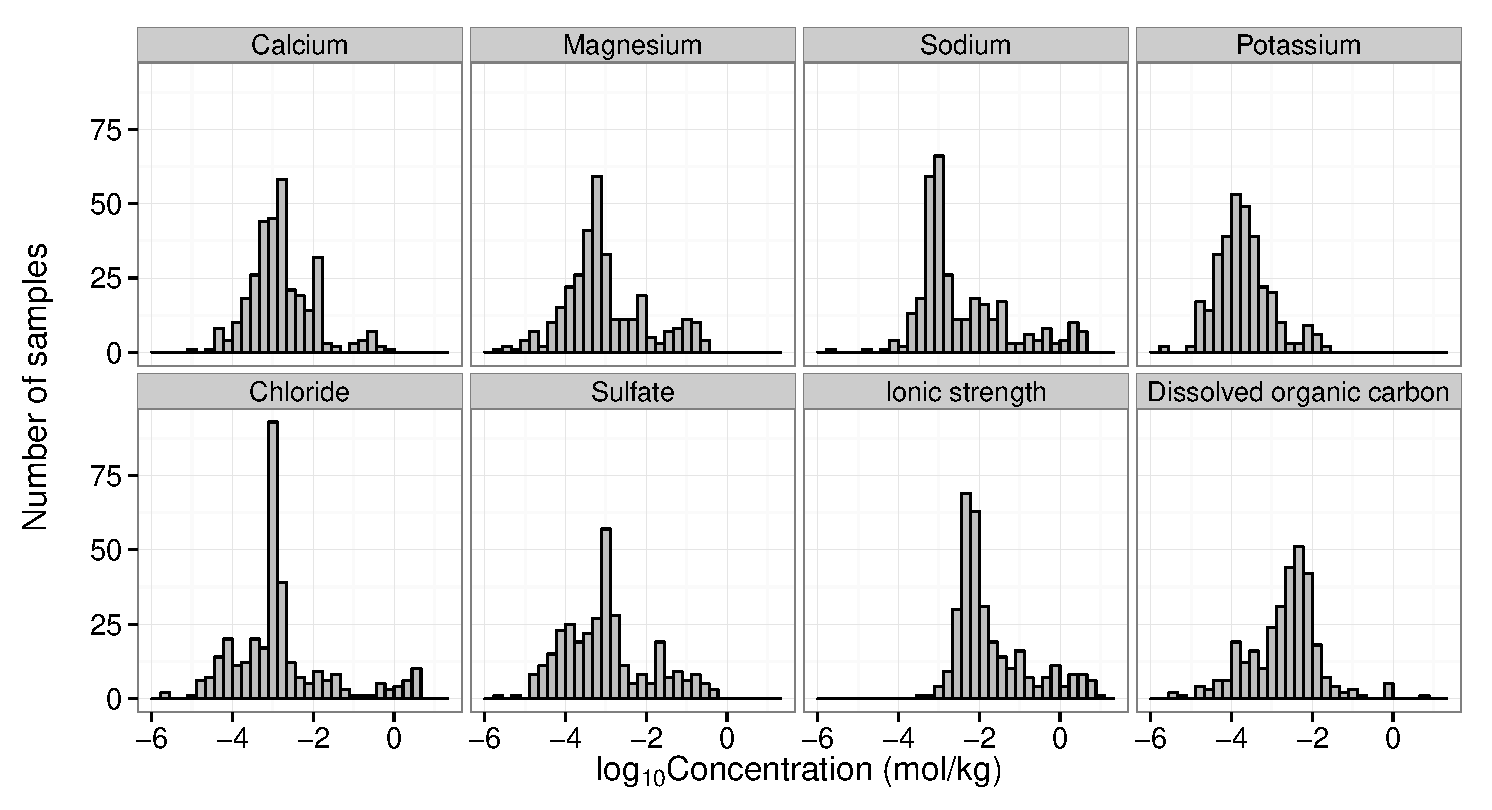
\includegraphics[width=\textwidth]{Ch3_figures/GW-chem-hist.pdf}
\caption{Major solution chemistry histograms for groundwater dataset. Total dissolved inorganic carbon was either given or estimated from alkalinity data using PHREEQC. Ionic strength was calculated using PHREEQC.}\label{fig:GW-chem-hist}
\end{center}
\end{figure}

\begin{figure}[htbp]
\begin{center}
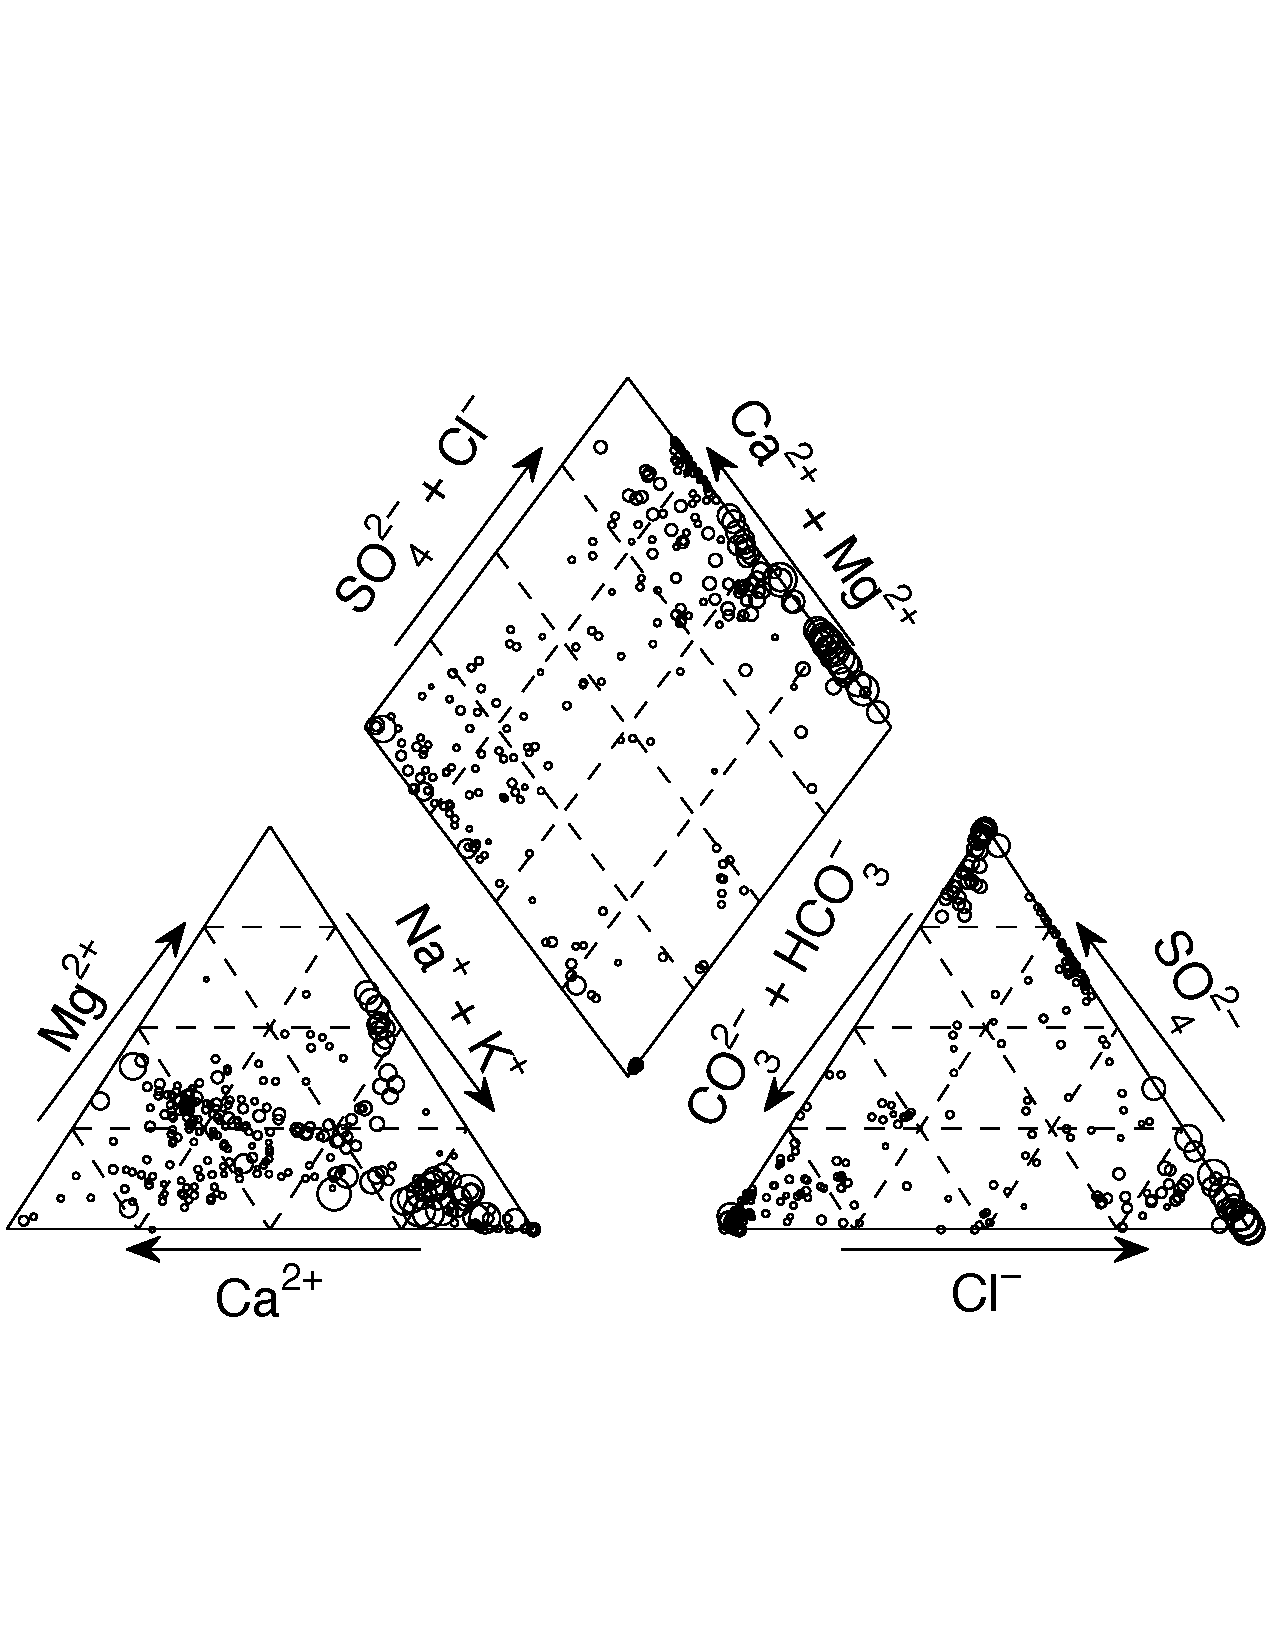
\includegraphics[width=0.67\textwidth]{Ch3_figures/GW-piper.pdf}
\caption{Piper diagram of ground water chemistry for circumneutral (5.5 $<$ pH $<$ 8.5) groundwater. Points scaled based on total dissolved solids. All plots range from 0 -- 100\%.}\label{fig:GW-chem-piper}
\end{center}
\end{figure}

Based on the available data three qualitative, rule-based water types were classified: fresh water ($N=122$; $6.5\leq$ pH $\leq8.5$; I $\leq0.1$ mol/kg), brines ($N=20$; $5.3\leq$ pH $\leq8.0$; I $\geq1.0$ mol/kg), and acidic waters ($N=63$; pH $<5.3$);
ionic strength and pH values were chosen to maximize data points within the various water classes while maintaining a reasonable bound on parameters.
Further subdivision of the freshwater data was possible (e.g. based on relative cation/anion composition) but was not pursued in favor of retaining a larger sample size.
The medians of the REE distributions of the classified groundwaters are shown in Figure~\ref{fig:GW-type-med}.

Utility of REE as tracers is reliant on identifying distinctive trends in different water types.
Of note in Figure~\ref{fig:GW-type-med} is the markedly higher concentrations of REE in acidic waters than either fresh water or brines, which supports the observations from Figure~\ref{fig:sum_vs_pH}, but also a deviation from the standard Oddo-Harkins effect pattern where Er and Yb are both less concentrated than their odd-numbered neighbors.
This effect was attributed to high degrees of censored or missing data for these elements (87\% for both Er and Yb in the acidic dataset) which leads to low-biased percentile estimates (as with Er and Yb) and large uncertainty (seen in all the HREE).
Despite showing little or no correlation with ionic strength (Figure~\ref{fig:REE-vs-major}) the REE, in particular the LREE and MREE, were more concentrated in brines than freshwater.

\begin{figure}[htbp]
\begin{center}
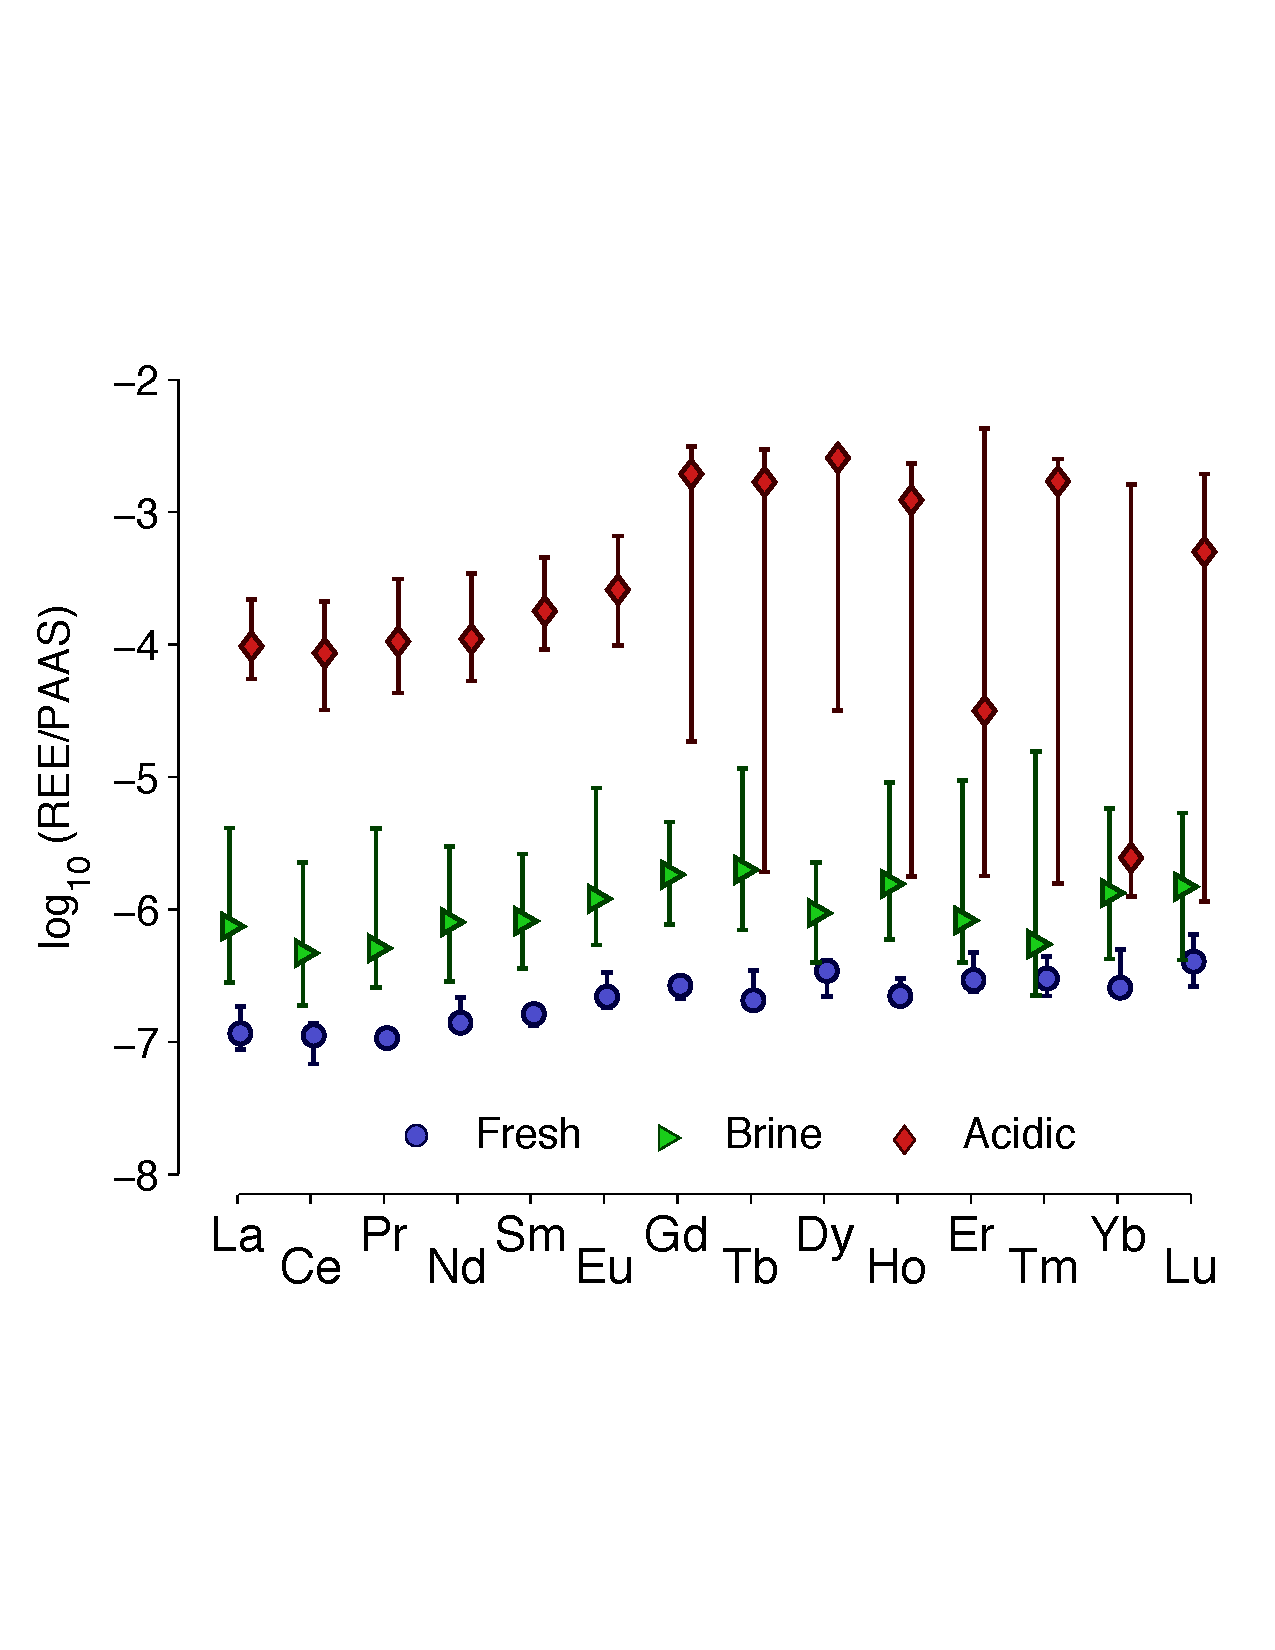
\includegraphics[width=0.67\textwidth]{Ch3_figures/REE-GW-KMmed.pdf}
\caption{Source-size weighted Kaplan-Meier estimates of median dissolved REE concentrations, normalized to Post-Archaean Average Shale (PAAS) values, in three characteristic groundwater types.
Error bars represent the 95\% confidence interval of the median.
Definitions of water classes are found in the text.
Estimates were made for individual elements, thus results do not represent a ``typical'' water sample across the REE suite.}\label{fig:GW-type-med}
\end{center}
\end{figure}

Understanding of the aqueous systematics of the REE is dominated by studies of fresh groundwaters, surface waters, and seawater.
Only 14\% of the groundwater data gathered had a calculated ionic strength of 1.0 mol/kg or greater (Figure~\ref{fig:I-ecdf}).
While thermodynamic models have been developed to predict REE aqueous speciation in brines \citep{Millero_GCA_1992},
the energetics of precipitation-dissolution and sorption-desorption in the REE system are not well defined for high ionic strength, chemically complex brines \citep{Quinn_MC_2006}.
Moreover, increased utilization of groundwater \citep{Chen_WRM_2013} in response to population growth, economic development, and climate change and the potential to exploit saline aquifers \citep{Benko_EES_2008} underscores the need to better understand the trace metal chemistry of brines.

\begin{figure}[htbp]
\begin{center}
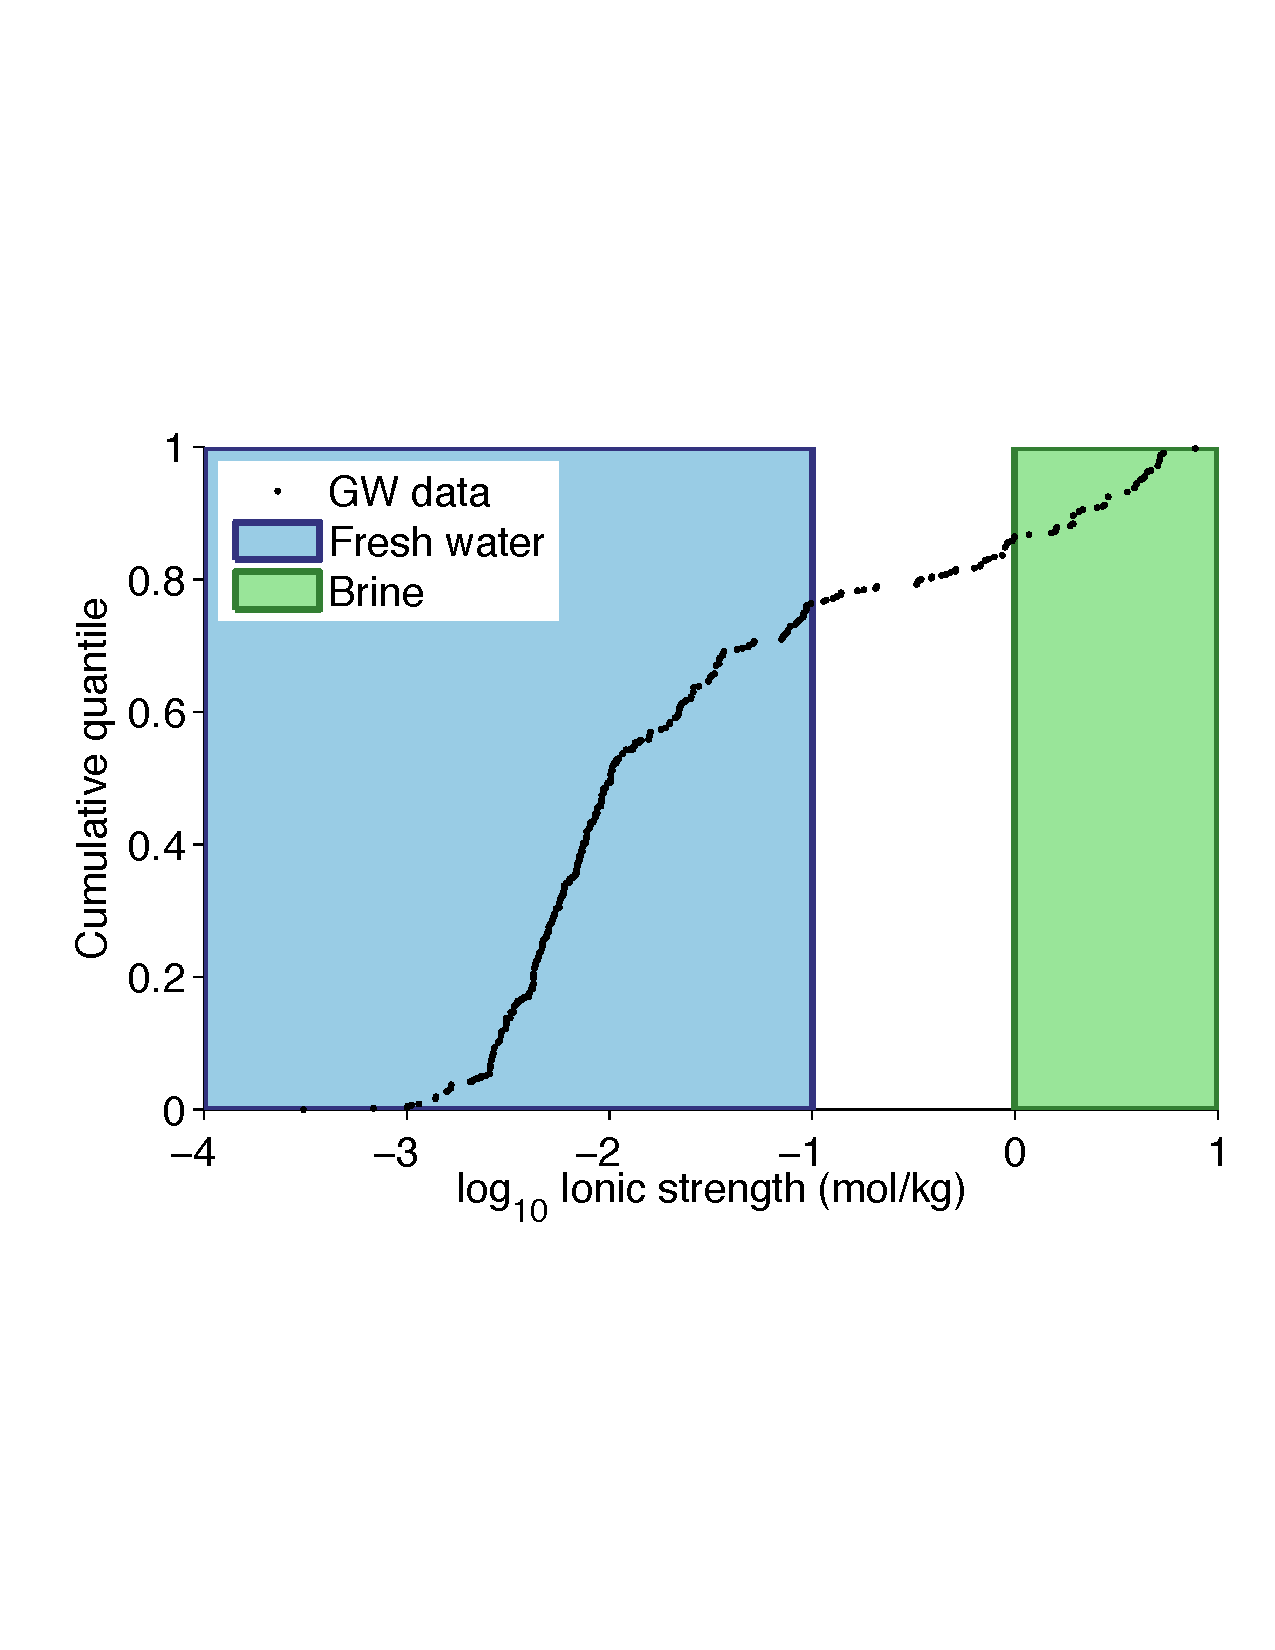
\includegraphics[width=0.67\textwidth]{Ch3_figures/GW-ionic-strength.pdf}
\caption{Source-size weighted, empirical cumulative distribution of calculated ionic strength in groundwater data set. Ionic strength calculated using PHREEQC \citep{PHREEQC}.}\label{fig:I-ecdf}
\end{center}
\end{figure}

Comparison of the HREE/MREE ratio to the MREE/LREE ratio succinctly captures the general shape of the REE profile of a sample, greatly simplifying visual comparison of samples.
Figure~\ref{fig:RDV-biplot} plots this scatter for classified groundwater data where all 14 REE were detected (39\% of the dataset).
For freshwater, more than 90\% of the samples exhibited MREE/LREE ratios greater than 1, with a median ratio of 1.74 and an IQR from 1.36 to 2.64.
HREE-MREE fractionation was more balanced with 53\% of samples having HREE/MREE ratios greater than 1, with a median ratio of 1.25 and an IQR from 0.64 to 1.6.
These data closely resemble the trends observed in the unclassified data set (not pictured), likely because freshwaters account for a large portion of the total data.
Fewer brine and acidic samples are available to plot, however brines appear to cluster with HREE enrichment, with all samples having MREE/LREE ratios greater than 1.0 and only 1 sample having HREE/MREE ratio less than 1.0, while acid samples exhibit convex-down profiles (MREE/LREE $> 1$ and HREE/MREE $< 1$).
However, it is difficult to ensure these are representative patterns given the small sample size for these water classes.

\begin{figure}[htbp]
\begin{center}
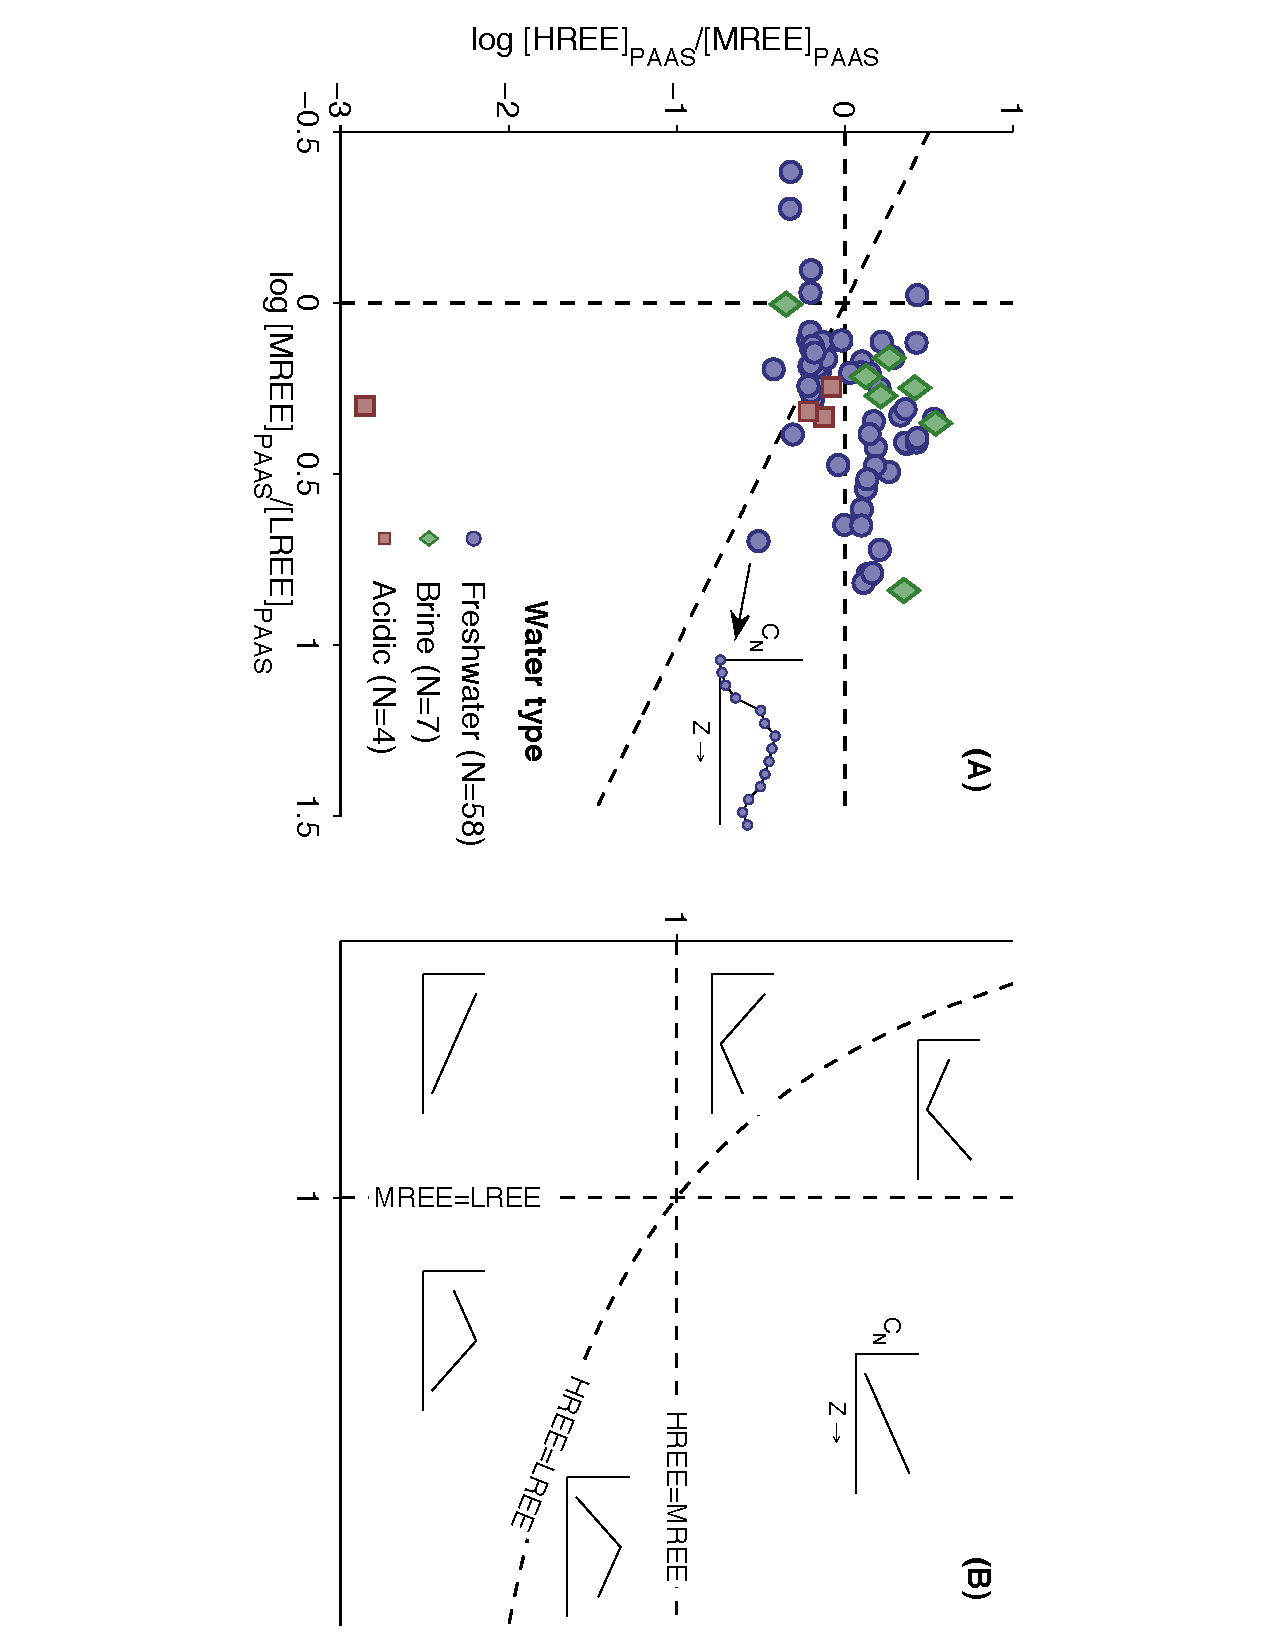
\includegraphics[width=\textwidth]{Ch3_figures/RDV-grouped-biplot.pdf}
\caption{(A) Averaged Post-Archaean Average Shale (PAAS) element ratio biplot for chemistry-classified groundwater data with no censoring, and (B) a schematic intended for interpretation, illustrating the general shape of the REE profile for a given sample.
Because each marker in (A) is a summary of the REE profile for an individual sample, an inset has been included to show the raw data (PAAS-normalized concentration, $C_N$, vs. elements in order of increasing atomic number, $Z$) for one sample.
The schematic in (B) is modified from Stolpe et al. \citep{Stolpe_GCA_2013} with permission.
Copyright 2013 Elsevier.
Note that the values in (A) have been log-transformed while the axes of the schematic are linear.}\label{fig:RDV-biplot}
\end{center}
\end{figure}

\subsection{Limitations of assembled dataset}

The primary goal of this analysis was to understand large-scale REE variability and trends.
However, researchers have understood that, because of complex geologies and watershed characteristics, there is significant merit in studying local, small-scale REE systematics.
This leads to specialized studies, for example, on the importance of colloids,33, 35, 42, 84, 87
phosphate complexation,12, 21, 91
or organic compounds.41, 85, 132-134 
While this approach yields crucial understanding of these processes, it also leads to a paucity of consistent data for inter-study comparison.
Moreover, it could motivate spurious extrapolation of thermodynamic or case study data to unique systems.

\bibliographystyle{unsrtnat}
\bibliography{Ch3_bib_edit}




